%%%%%%%%%%%%%%%%%%%%%%%%%%%%%%%%%%%%%%%%%%%%%%%%%%%%%%%%%%%%%%%%%%%%%%
%%%%%%%%%%%%%%%%%%%%%%%%%%%%%%%%%%%%%%%%%%%%%%%%%%%%%%%%%%%%%%%%%%%%%%
%%
%% IVT LaTeX template
%%   Kirill Müller
%%   kirill.mueller@ivt.baug.ethz.ch
%%
%%%%%%%%%%%%%%%%%%%%%%%%%%%%%%%%%%%%%%%%%%%%%%%%%%%%%%%%%%%%%%%%%%%%%%
%%%%%%%%%%%%%%%%%%%%%%%%%%%%%%%%%%%%%%%%%%%%%%%%%%%%%%%%%%%%%%%%%%%%%%

%%%%%%%%%%%%%%%%%%%%%%%%%%%%%%%%%%%%%%%%%%%%%%%%%%%%%%%%%%%%%%%%%%%%%%
%%%%%%%%%%%%%%%%%%%%%%%%%%%%%%%%%%%%%%%%%%%%%%%%%%%%%%%%%%%%%%%%%%%%%%
%%
%% Encoding check:
%%   ä  ö  ü  Ä  Ö  Ü  ß  á  é  í  ó  ú  à  è  ì  ò  ù  â  ê  î  ô  û
%%
%%   If the above contains rubbish, please re-open this file using
%%   one of the following encodings: Latin1, ISO-8859-1, Windows-1252.
%%   DO NOT save the file in this case!
%%
%%%%%%%%%%%%%%%%%%%%%%%%%%%%%%%%%%%%%%%%%%%%%%%%%%%%%%%%%%%%%%%%%%%%%%
%%%%%%%%%%%%%%%%%%%%%%%%%%%%%%%%%%%%%%%%%%%%%%%%%%%%%%%%%%%%%%%%%%%%%%

%%%%%%%%%%%%%%%%%%%%%%%%%%%%%%%%%%%%%%%%%%%%%%%%%%%%%%%%%%%%%%%%%%%%%%
%%%%%%%%%%%%%%%%%%%%%%%%%%%%%%%%%%%%%%%%%%%%%%%%%%%%%%%%%%%%%%%%%%%%%%
%%
%% This is an example for writing a paper at the IVT.
%% It supports English and German language.
%% By using it, it is possible to switch paper layouts easily
%% (e.g., working paper style into TRB style)
%%
%% The easiest way to write you own paper is to create an
%% appropriate directory stucture in the papers subdirectory
%% i.e. papers/strc/2007/mypaper,
%% copy this template and modify it there.
%%
%% See the note below on renaming the main file.
%%
%% Each keyword is documented. Just follow the instructions...
%% Enjoy!
%%
%%%%%%%%%%%%%%%%%%%%%%%%%%%%%%%%%%%%%%%%%%%%%%%%%%%%%%%%%%%%%%%%%%%%%%
%%%%%%%%%%%%%%%%%%%%%%%%%%%%%%%%%%%%%%%%%%%%%%%%%%%%%%%%%%%%%%%%%%%%%%

%%%%%%%%%%%%%%%%%%%%%%%%%%%%%%%%%%%%%%%%%%%%%%%%%%%%%%%%%%%%%%%%%%%%%%
%%%%%%%%%%%%%%%%%%%%%%%%%%%%%%%%%%%%%%%%%%%%%%%%%%%%%%%%%%%%%%%%%%%%%%
%%
%% IMPORTANT NOTE ON FILE RENAMES:
%%   If you rename this file, look for the text "Template"
%%   in all files and change this to the new filename, too.
%%   There is a script that will do this for you in
%%   Linux/Windows+cygwin or Mac OS X: Simply execute
%%
%%       _latexfiles/tools/rename.sh Template NewName
%%
%%   Substitute NewName with a name of your choice.
%%
%%   In Windows, use your favorite find-in-text-files tool
%%
%%%%%%%%%%%%%%%%%%%%%%%%%%%%%%%%%%%%%%%%%%%%%%%%%%%%%%%%%%%%%%%%%%%%%%
%%%%%%%%%%%%%%%%%%%%%%%%%%%%%%%%%%%%%%%%%%%%%%%%%%%%%%%%%%%%%%%%%%%%%%

%%%%%%%%%%%%%%%%%%%%%%%%%%%%%%%%%%%%%%%%%%%%%%%%%%%%%%%%%%%%%%%%%%%%%%
%% Location of the common files
%%   If unsure, please leave this as it is
\newcommand{\mypath}{_latexfiles/}
%\newcommand{\mypath}{../../../}
%%%%%%%%%%%%%%%%%%%%%%%%%%%%%%%%%%%%%%%%%%%%%%%%%%%%%%%%%%%%%%%%%%%%%%

%%%%%%%%%%%%%%%%%%%%%%%%%%%%%%%%%%%%%%%%%%%%%%%%%%%%%%%%%%%%%%%%%%%%%%
%% language specification:
%%   Here you define in which langugage your paper will be written.
%%   There are ALWAYS 2 languages to define (even you do not need it.)
%%   Since we are writing only in German or English, other languages
%%   are not supported.
%%   Choose either 'german' or 'english' as your first language.
\newcommand{\myfirstlang}{english}
%%%%%%%%%%%%%%%%%%%%%%%%%%%%%%%%%%%%%%%%%%%%%%%%%%%%%%%%%%%%%%%%%%%%%%

%%%%%%%%%%%%%%%%%%%%%%%%%%%%%%%%%%%%%%%%%%%%%%%%%%%%%%%%%%%%%%%%%%%%%%
%% Include Paper-Layout:
%%   Here the ivt working paper layout is chosen
%%   For changing this paper into i.e. TRB layout just change "ivt-wp"
%%   to "trb"
% !TeX encoding = usascii
% Prepare to get rid of \mypath one day
\providecommand\mypath[3]{}
%%%%%%%%%%%%%%%%%%%%%%%%%%%%%%%%%%%%%%%%%%%%%%%%%%%%%%%%%%%%%%%%%%%%%%
%% $Id: trb-lineNumbered.tex 12326 2013-10-11 10:04:04Z muelleki $
%%%%%%%%%%%%%%%%%%%%%%%%%%%%%%%%%%%%%%%%%%%%%%%%%%%%%%%%%%%%%%%%%%%%%%

%%%%%%%%%%%%%%%%%%%%%%%%%%%%%%%%%%%%%%%%%%%%%%%%%%%%%%%%%%%%%%%%%%%%%%
%%
%% TRB PAPER LAYOUT
%% Date: 2007-06-28
%% author:
%%   Michael Balmer, balmer@ivt.baug.ethz.ch
%%
%%%%%%%%%%%%%%%%%%%%%%%%%%%%%%%%%%%%%%%%%%%%%%%%%%%%%%%%%%%%%%%%%%%%%%

% !TeX encoding = usascii
% Prepare to get rid of \mypath one day
\providecommand\mypath[3]{}
%%%%%%%%%%%%%%%%%%%%%%%%%%%%%%%%%%%%%%%%%%%%%%%%%%%%%%%%%%%%%%%%%%%%%%
%% $Id: trb.tex 17089 2016-08-10 09:29:01Z muelleki $
%%%%%%%%%%%%%%%%%%%%%%%%%%%%%%%%%%%%%%%%%%%%%%%%%%%%%%%%%%%%%%%%%%%%%%

%%%%%%%%%%%%%%%%%%%%%%%%%%%%%%%%%%%%%%%%%%%%%%%%%%%%%%%%%%%%%%%%%%%%%%
%%
%% TRB PAPER LAYOUT
%% Date: 2007-06-28
%% author:
%%   Michael Balmer, balmer@ivt.baug.ethz.ch
%%
%%%%%%%%%%%%%%%%%%%%%%%%%%%%%%%%%%%%%%%%%%%%%%%%%%%%%%%%%%%%%%%%%%%%%%

%%%%%%%%%%%%%%%%%%%%%%%%%%%%%%%%%%%%%%%%%%%%%%%%%%%%%%%%%%%%%%%%%%%%%%
%%%%%%%%%%%%%%%%%%%%%%%%%%%%%%%%%%%%%%%%%%%%%%%%%%%%%%%%%%%%%%%%%%%%%%
%%
%% Standard latex layout configurations
%%   Here, commands and settings are use which are available
%%   by the latex packages
%%
%%%%%%%%%%%%%%%%%%%%%%%%%%%%%%%%%%%%%%%%%%%%%%%%%%%%%%%%%%%%%%%%%%%%%%
%%%%%%%%%%%%%%%%%%%%%%%%%%%%%%%%%%%%%%%%%%%%%%%%%%%%%%%%%%%%%%%%%%%%%%
%% Type of document:
%% - Paperformat: letterpaper, a4paper, a5paper, b5paper,
%%   executivepaper, legalpaper
%% - Main font size: 10pt, 11pt, 12pt
%% - Formulae setting: - (centred), fleqn (left-aligned)
%% - Numbering of formulae: - (right-aligned), leqno (left-aligned)
%% - New page after title: titlepage, notitlepage
%% - Number of columns per page: onecolumn, twocolumn
%% - Page style: oneside, twoside
%% - Paper rotation: - (protrait), landscape
%% - Chapter start: openright, openany (not required for oneside layout)
%% - Mark overfull boxes: draft, final
\documentclass[12pt,fleqn,titlepage,onecolumn,oneside,final]{article}
%%%%%%%%%%%%%%%%%%%%%%%%%%%%%%%%%%%%%%%%%%%%%%%%%%%%%%%%%%%%%%%%%%%%%%
%% borders, margrins and offset
\usepackage[a4paper,left=1.0in,right=1.0in,top=1.0in,bottom=1.0in]{geometry}
%%%%%%%%%%%%%%%%%%%%%%%%%%%%%%%%%%%%%%%%%%%%%%%%%%%%%%%%%%%%%%%%%%%%%%
%% Package options
\PassOptionsToPackage{nooneline,font=bf,labelsep=quad,format=hang}{caption}
\PassOptionsToPackage{font=small,labelsep=space}{subcaption}
\PassOptionsToPackage{fleqn}{amsmath}
\PassOptionsToPackage{compress}{natbib}
\PassOptionsToPackage{noabbrev}{cleveref}
%%%%%%%%%%%%%%%%%%%%%%%%%%%%%%%%%%%%%%%%%%%%%%%%%%%%%%%%%%%%%%%%%%%%%%
%% Include default packages and settings
%%%%%%%%%%%%%%%%%%%%%%%%%%%%%%%%%%%%%%%%%%%%%%%%%%%%%%%%%%%%%%%%%%%%%%
%% Bugfixes:
\ifdefined\ivtnofixltx\else\usepackage{fixltx2e}\fi
%%%%%%%%%%%%%%%%%%%%%%%%%%%%%%%%%%%%%%%%%%%%%%%%%%%%%%%%%%%%%%%%%%%%%%
%% Smart space after macro:
\usepackage{xspace}
%%%%%%%%%%%%%%%%%%%%%%%%%%%%%%%%%%%%%%%%%%%%%%%%%%%%%%%%%%%%%%%%%%%%%%
%% string manipulation
\usepackage{stringstrings}
\usepackage{textcase}
%%%%%%%%%%%%%%%%%%%%%%%%%%%%%%%%%%%%%%%%%%%%%%%%%%%%%%%%%%%%%%%%%%%%%%
%% providing if-then-else command:
\usepackage{ifthen}
%%%%%%%%%%%%%%%%%%%%%%%%%%%%%%%%%%%%%%%%%%%%%%%%%%%%%%%%%%%%%%%%%%%%%%
%% providing expandonce command (and others):
\usepackage{etoolbox}
%%%%%%%%%%%%%%%%%%%%%%%%%%%%%%%%%%%%%%%%%%%%%%%%%%%%%%%%%%%%%%%%%%%%%%
%% LaTeX3 document parsing:
\usepackage{xparse}
%%%%%%%%%%%%%%%%%%%%%%%%%%%%%%%%%%%%%%%%%%%%%%%%%%%%%%%%%%%%%%%%%%%%%%
%% helper commands
\newcommand{\ifeqe}[4]{%
  \ifthenelse{\equal{\expandonce{#1}}{\expandonce{#2}}}{#3}{#4}%
}
\newcommand{\ifeq}[3]{%
  \ifeqe{#1}{#2}{#3}{}%
}
\newcommand{\ifneq}[3]{%
  \ifeqe{#1}{#2}{}{#3}%
}
\newcommand{\ifne}[2]{%
  \ifneq{#1}{}{#2}%
}
%%%%%%%%%%%%%%%%%%%%%%%%%%%%%%%%%%%%%%%%%%%%%%%%%%%%%%%%%%%%%%%%%%%%%%
%% number of words used (wordcount)
%% - include number
\AtBeginDocument{%
\providecommand{\mywordcount}{}%
\renewcommand{\mywordcount}{%
  \newcounter{mywordcount}%
  \IfFileExists{mywordcount}{%
    \input{mywordcount}%
    \setcounter{mywordcount}{\mytextwordcount}%
  }{%
    \newcommand{\mytextwordcount}{Use the script wordcount.py to count}%
  }%
  \newcounter{myequivalentcount}%
  \setcounter{myequivalentcount}{\arabic{mywordcount} + \totvalue{figure} * 250 + \totvalue{table} * 250}%
  \ifthenelse{\equal{\totvalue{table}}{0}}{%
    \newcommand{\mytableid}{}%
  }{%
    \ifthenelse{\equal{\totvalue{table}}{1}}{%
      \newcommand{\mytableid}{ + 1 table}%
    }{%
      \newcommand{\mytableid}{ + \total{table}\xspace tables}%
    }%
  }%
  \ifthenelse{\equal{\totvalue{figure}}{0}}{%
    \newcommand{\myfigureid}{}%
  }{%
    \ifthenelse{\equal{\totvalue{figure}}{1}}{%
      \newcommand{\myfigureid}{ + 1 figure}%
    }{%
      \newcommand{\myfigureid}{ + \total{figure}\xspace figures}%
    }%
  }%
  \ifthenelse{\equal{\arabic{mywordcount}}{\arabic{myequivalentcount}}}{%
    \newcommand{\myeqtext}{}
  }{%
    \newcommand{\myeqtext}{ = \arabic{myequivalentcount} word equivalents}
  }%
  \mytextwordcount\xspace words\myfigureid\mytableid\myeqtext%
}%
}
\newcommand{\ifelsewc}[2]{%
  \ifdefined\wcFileName%
    #1%
  \else%
    #2%
  \fi%
}
\newcommand{\ifwc}[1]{%
  \ifelsewc{#1}{}%
}
\newcommand{\ifnwc}[1]{%
  \ifelsewc{}{#1}%
}
%%%%%%%%%%%%%%%%%%%%%%%%%%%%%%%%%%%%%%%%%%%%%%%%%%%%%%%%%%%%%%%%%%%%%%
%% Support for conversion to Word
\providecommand{\AsPicture}[1]{#1}
\makeatletter
\@ifpackageloaded{tex4ht}{%
  \newcommand{\ifelseht}[2]{#1}%
}{%
  \newcommand{\ifelseht}[2]{#2}%
}%
\makeatother
\newcommand{\ifht}[1]{%
  \ifelseht{#1}{}%
}
\newcommand{\ifnht}[1]{%
  \ifelseht{}{#1}%
}
%%%%%%%%%%%%%%%%%%%%%%%%%%%%%%%%%%%%%%%%%%%%%%%%%%%%%%%%%%%%%%%%%%%%%%
%% Support for make parts of the document (such as page headers)
%% non-selectable
%%   (usually, you also want to ignore these parts when counting
%%    words)
\ifelseht{%
  \DeclareRobustCommand\squelch[1]{#1}%
}{%
  \ifelsewc{%
    \DeclareRobustCommand\squelch[1]{}%
  }{%
    \usepackage{accsupp}
    \DeclareRobustCommand\squelch[1]{%
      \BeginAccSupp{method=plain,ActualText={}}#1\EndAccSupp{}}%
  }
}%
%%%%%%%%%%%%%%%%%%%%%%%%%%%%%%%%%%%%%%%%%%%%%%%%%%%%%%%%%%%%%%%%%%%%%%
%% Table captions aligned with table:
\usepackage{varwidth}
%%%%%%%%%%%%%%%%%%%%%%%%%%%%%%%%%%%%%%%%%%%%%%%%%%%%%%%%%%%%%%%%%%%%%%
%% default language:
\ifthenelse{\equal{\myfirstlang}{german}}{%
  \usepackage[english,german]{babel}%
}{%
  \usepackage[german,english]{babel}%
}
%%%%%%%%%%%%%%%%%%%%%%%%%%%%%%%%%%%%%%%%%%%%%%%%%%%%%%%%%%%%%%%%%%%%%%
%% bibliography:
\usepackage{natbib}
%%%%%%%%%%%%%%%%%%%%%%%%%%%%%%%%%%%%%%%%%%%%%%%%%%%%%%%%%%%%%%%%%%%%%%
%% AMS mathematics:
%%   (include before txfonts, and use txfonts's iint)
\usepackage{amsmath}
\ifnwc{%
  \let\iint\relax
}%
%%%%%%%%%%%%%%%%%%%%%%%%%%%%%%%%%%%%%%%%%%%%%%%%%%%%%%%%%%%%%%%%%%%%%%
%% The package microtype adjusts font width for individual words
%%   in order to achieve better line breaking.
%%   Also, margin kerning makes the margin look more even.
%%   This also renders the use of \sloppy unnecessary.
\usepackage{microtype}
\fussy
%%%%%%%%%%%%%%%%%%%%%%%%%%%%%%%%%%%%%%%%%%%%%%%%%%%%%%%%%%%%%%%%%%%%%%
%% providing umlauts:
\usepackage[utf8]{inputenc}
\ifnwc{%
\usepackage[T1]{fontenc}
}
%%%%%%%%%%%%%%%%%%%%%%%%%%%%%%%%%%%%%%%%%%%%%%%%%%%%%%%%%%%%%%%%%%%%%%
%% line spacing
\ifnwc{%
\usepackage{setspace}
}
%%%%%%%%%%%%%%%%%%%%%%%%%%%%%%%%%%%%%%%%%%%%%%%%%%%%%%%%%%%%%%%%%%%%%%
%% Allow rotating single pages
%% The package is orientated correctly when displayed on screen
\usepackage{pdflscape}
%% Extract command from this package, to be used in the
%% "sidewaysfigure" environment...
\makeatletter
\let\AddPageRotate=\PLS@AddRotate
\let\RemovePageRotate=\PLS@RemoveRotate
\makeatother
%% ...but reset the command that un-rotates pages inside the
%% "landscape" environment, so that the page rotation stays in effect
%% there
%%
%% (AtBeginEnvironment
\ifdefined\AtBeginEnvironment
  \AtBeginEnvironment{landscape}{\def\RemovePageRotate{\relax}}
\else
  \message{Use a recent version of etoolbox package to get
  correct page rotation in the landscape environment.}
\fi
%%%%%%%%%%%%%%%%%%%%%%%%%%%%%%%%%%%%%%%%%%%%%%%%%%%%%%%%%%%%%%%%%%%%%%
%% Hack for orientating sideways{tables,figures} correctly
%%
%% By default, every page is not rotated:
\usepackage{everypage}
\AddEverypageHook{\RemovePageRotate}%
%% The package floatpag implements a hook that is executed
%% when the current float is displayed. We use this hook
%% to add an \AddPageRotate command for the sideways floats.
\usepackage{floatpag}
\ifnwc{%
  \AtBeginDocument{%
    \pagestyle{\mypagestyle}%
    \floatpagestyle{\mypagestyle}%
    \rotfloatpagestyle{\mypagestyle}%
  }
}
\makeatletter
\def\thisfloatcommand#1{%
  \expandafter\expandafter\expandafter\gdef\expandafter\csname\number\@currbox @float\endcsname{#1}\relax}
\makeatother
%%%%%%%%%%%%%%%%%%%%%%%%%%%%%%%%%%%%%%%%%%%%%%%%%%%%%%%%%%%%%%%%%%%%%%
%% Captions and subcaptions
\usepackage{caption}
\ifnht{%
  \usepackage[singlelinecheck=on,labelformat=simple]{subcaption}
  \renewcommand\thesubfigure{(\alph{subfigure})}
  \renewcommand\thesubtable{(\alph{subtable})}
}
%%%%%%%%%%%%%%%%%%%%%%%%%%%%%%%%%%%%%%%%%%%%%%%%%%%%%%%%%%%%%%%%%%%%%%
%% providing graphics:
\usepackage{graphics}
\usepackage{graphicx}
%%%%%%%%%%%%%%%%%%%%%%%%%%%%%%%%%%%%%%%%%%%%%%%%%%%%%%%%%%%%%%%%%%%%%%
%% sideways figures and tables:
\usepackage[figuresright]{rotating}
%%%%%%%%%%%%%%%%%%%%%%%%%%%%%%%%%%%%%%%%%%%%%%%%%%%%%%%%%%%%%%%%%%%%%%
%% figures:
%%   The following are sometimes needed to avoid pushing
%%   the figs to the end of the text.
\def\textfraction{0.0}
\def\topfraction{0.9999}
\def\dbltopfraction{0.9999}
\def\floatpagefraction{0.8}
%%%%%%%%%%%%%%%%%%%%%%%%%%%%%%%%%%%%%%%%%%%%%%%%%%%%%%%%%%%%%%%%%%%%%%
%% tables:
\usepackage{multirow}
%%%%%%%%%%%%%%%%%%%%%%%%%%%%%%%%%%%%%%%%%%%%%%%%%%%%%%%%%%%%%%%%%%%%%%
%% pretty printing:
\usepackage{listings}
%%%%%%%%%%%%%%%%%%%%%%%%%%%%%%%%%%%%%%%%%%%%%%%%%%%%%%%%%%%%%%%%%%%%%%
%% XML code setup:
\lstloadlanguages{XML}
%%
\lstset {
  columns=fullflexible,
  showstringspaces=false,
  basicstyle=\ttfamily\footnotesize,
  lineskip=0pt,
  breaklines=true,
  breakatwhitespace=true,
  breakindent=12pt,
  fontadjust=true,
  keywordstyle=\bfseries,
  commentstyle=\itshape,
  stringstyle=\bfseries\itshape,
  xleftmargin=0mm,
  xrightmargin=0mm,
  tabsize=2
}

\lstdefinelanguage{XML}
{
  morestring=[b]",
  moredelim=[s][\bfseries\color{Maroon}]{<}{\ },
  moredelim=[s][\bfseries\color{Maroon}]{</}{>},
  moredelim=[l][\bfseries\color{Maroon}]{/>},
  moredelim=[l][\bfseries\color{Maroon}]{>},
  morecomment=[s]{<?}{?>},
  morecomment=[s]{<!--}{-->},
  commentstyle=\color{DarkOliveGreen},
  stringstyle=\color{blue},
  identifierstyle=\color{red}
}
%%%%%%%%%%%%%%%%%%%%%%%%%%%%%%%%%%%%%%%%%%%%%%%%%%%%%%%%%%%%%%%%%%%%%%
%% Support for figure and table count:
\usepackage{totcount}
\usepackage{calc}
\regtotcounter{figure}
\regtotcounter{table}
%%%%%%%%%%%%%%%%%%%%%%%%%%%%%%%%%%%%%%%%%%%%%%%%%%%%%%%%%%%%%%%%%%%%%%
%% Less space between enumeration lists
\usepackage{paralist}
\renewenvironment{itemize}[1]{\begin{compactitem}#1}{\end{compactitem}}
\renewenvironment{enumerate}[1]{\begin{compactenum}#1}{\end{compactenum}}
\renewenvironment{description}[0]{\begin{compactdesc}}{\end{compactdesc}}
%%%%%%%%%%%%%%%%%%%%%%%%%%%%%%%%%%%%%%%%%%%%%%%%%%%%%%%%%%%%%%%%%%%%%%
%% Typesetting-quality tables
\usepackage{booktabs}
%%%%%%%%%%%%%%%%%%%%%%%%%%%%%%%%%%%%%%%%%%%%%%%%%%%%%%%%%%%%%%%%%%%%%%
%% new verbatim environment
\usepackage{verbatim}
%%%%%%%%%%%%%%%%%%%%%%%%%%%%%%%%%%%%%%%%%%%%%%%%%%%%%%%%%%%%%%%%%%%%%%
%% Extended color definitions
\PassOptionsToPackage{svgnames}{xcolor}
\usepackage{xcolor}
%%%%%%%%%%%%%%%%%%%%%%%%%%%%%%%%%%%%%%%%%%%%%%%%%%%%%%%%%%%%%%%%%%%%%%
%% Just in case (before hyperref):
\usepackage{float}
\usepackage{longtable}
\usepackage{ltabptch}
\usepackage{nameref}
%%%%%%%%%%%%%%%%%%%%%%%%%%%%%%%%%%%%%%%%%%%%%%%%%%%%%%%%%%%%%%%%%%%%%%
%% Use hyper-refs for URLs and citations,
%% allow line breaks for URLs
%%   include after all other packages, especially after titlesec
\PassOptionsToPackage{obeyspaces}{url}
\ifnht{\usepackage{hyperref}}
\usepackage{url}
%%%%%%%%%%%%%%%%%%%%%%%%%%%%%%%%%%%%%%%%%%%%%%%%%%%%%%%%%%%%%%%%%%%%%%
%% convenient referencing (after hyperref):
\usepackage[capitalize]{cleveref}
%%%%%%%%%%%%%%%%%%%%%%%%%%%%%%%%%%%%%%%%%%%%%%%%%%%%%%%%%%%%%%%%%%%%%%
%% tables (after hyperref):
\usepackage{tabularx}
%%%%%%%%%%%%%%%%%%%%%%%%%%%%%%%%%%%%%%%%%%%%%%%%%%%%%%%%%%%%%%%%%%%%%%
%% do not count words in references
%% count only title, subtitle and abstract, no auxiliary information
\ifwc{%
  \renewcommand{\bibliography}[1]{}%
  \AtBeginDocument{%
    \renewcommand{\createtitlepage}{\mytitle \mysubtitle}%
    \renewcommand{\createabstract}[1]{#1}%
  }%
}
%%%%%%%%%%%%%%%%%%%%%%%%%%%%%%%%%%%%%%%%%%%%%%%%%%%%%%%%%%%%%%%%%%%%%%
%% for document classes that do not provide \captionabove and
%% \captionbelow
\providecommand{\captionabove}[2][]{\caption[#1]{#2}}
\providecommand{\captionbelow}[2][]{\caption[#1]{#2}}

%%%%%%%%%%%%%%%%%%%%%%%%%%%%%%%%%%%%%%%%%%%%%%%%%%%%%%%%%%%%%%%%%%%%%%
%% Header and footer definition:
\usepackage{fancyhdr}%
\newcommand{\mypagestyle}{fancy}
\fancyhf{}%
\fancyhead[R]{\footnotesize \squelch{\nouppercase{\thepage}}}%
\fancyhead[L]{\footnotesize \squelch{\nouppercase{\internauthorstring}}}%
\renewcommand{\headrulewidth}{0pt}%
\renewcommand{\footrulewidth}{0pt}%
%%%%%%%%%%%%%%%%%%%%%%%%%%%%%%%%%%%%%%%%%%%%%%%%%%%%%%%%%%%%%%%%%%%%%%
%% paragraph settings:
\setlength{\parindent}{\parindent}%
\setlength{\parskip}{6pt}
%%%%%%%%%%%%%%%%%%%%%%%%%%%%%%%%%%%%%%%%%%%%%%%%%%%%%%%%%%%%%%%%%%%%%%
%% caption settings:
\DeclareCaptionLabelFormat{allcaps}{\MakeUppercase{#1\ #2}}
\captionsetup*{labelformat=allcaps}
%%%%%%%%%%%%%%%%%%%%%%%%%%%%%%%%%%%%%%%%%%%%%%%%%%%%%%%%%%%%%%%%%%%%%%
%% Define the depth of numbering parts,chapter,sections and paragraphs:
%%   Numbers representing the depth of sectional units:
%%   -1 = \part    (in book or report document classes)
%%    0 = \chapter (in book or report document classes)
%%    0 = \part    (in article document classes)
%%    1 = \section
%%    2 = \subsection
%%    3 = \subsubsection
%%    4 = \paragraph
%%    5 = \subparagraph
\setcounter{secnumdepth}{3}
%%%%%%%%%%%%%%%%%%%%%%%%%%%%%%%%%%%%%%%%%%%%%%%%%%%%%%%%%%%%%%%%%%%%%%
%% citation style:
\setcitestyle{numbers}
\bibpunct{\textit\bgroup(}{)\egroup}{,}{n}{,}{,}
\providecommand{\citenumfont}[1]{}
\renewcommand{\citenumfont}[1]{\textit{#1}}
\renewcommand{\bibnumfmt}[1]{#1.}
\ifthenelse{\equal{\myfirstlang}{german}}{%
  \bibliographystyle{\mypath../_latexfiles/styles/template_ivt-unsrt-ger}%
}{%
  \bibliographystyle{\mypath../_latexfiles/styles/template_ivt-unsrt-eng}%
}
%%%%%%%%%%%%%%%%%%%%%%%%%%%%%%%%%%%%%%%%%%%%%%%%%%%%%%%%%%%%%%%%%%%%%%
%% no indentation for formulae:
\setlength\mathindent{0pt}
%%%%%%%%%%%%%%%%%%%%%%%%%%%%%%%%%%%%%%%%%%%%%%%%%%%%%%%%%%%%%%%%%%%%%%
%% Times font
% !TeX encoding = usascii
%%%%%%%%%%%%%%%%%%%%%%%%%%%%%%%%%%%%%%%%%%%%%%%%%%%%%%%%%%%%%%%%%%%%%%
%% Font:
%% (unfortunately, mathptmx does not provide bold math fonts,
%%  and times still uses the rather different CM font for maths)
\ifnwc{%
  \ifnht{%
    \usepackage{newtxtext}
    \usepackage{newtxmath}
    \usepackage{courier}
    \undef\oct
  }
}


%%%%%%%%%%%%%%%%%%%%%%%%%%%%%%%%%%%%%%%%%%%%%%%%%%%%%%%%%%%%%%%%%%%%%%
%% single line spacing
\singlespacing
%%%%%%%%%%%%%%%%%%%%%%%%%%%%%%%%%%%%%%%%%%%%%%%%%%%%%%%%%%%%%%%%%%%%%%
%% heading settings:
%%   now using the titlesec package
\usepackage{titlesec}
%%
%% legacy (match appearance of previous version)
\newlength{\sectionbeforedist}
\setlength{\sectionbeforedist}{\parskip}
\addtolength{\sectionbeforedist}{1.16ex}
%%
%% section
\titleformat{\section}{\normalfont\bfseries}{}{0pt}{\MakeUppercase}
\titlespacing*{\section}{0in}{\sectionbeforedist}{0.001pt}
%%
%% subsection
\titleformat{\subsection}{\normalfont\bfseries}{}{0pt}{}
\titlespacing*{\subsection}{0in}{\sectionbeforedist}{0.001pt}
%%
%% subsubsection
\titleformat{\subsubsection}{\normalfont\itshape}{}{0pt}{}
\titlespacing*{\subsubsection}{0in}{\sectionbeforedist}{0.001pt}
%%
%% paragraph
\titleformat{\paragraph}[runin]{\normalfont\bfseries}{}{0pt}{}
\titlespacing*{\paragraph}{0in}{\sectionbeforedist}{5pt}
%%
%% subparagraph
\titleformat{\subparagraph}[runin]{\normalfont\itshape}{}{0pt}{}
\titlespacing*{\subparagraph}{0in}{\sectionbeforedist}{5pt}
%%%%%%%%%%%%%%%%%%%%%%%%%%%%%%%%%%%%%%%%%%%%%%%%%%%%%%%%%%%%%%%%%%%%%%

%%%%%%%%%%%%%%%%%%%%%%%%%%%%%%%%%%%%%%%%%%%%%%%%%%%%%%%%%%%%%%%%%%%%%%
%%%%%%%%%%%%%%%%%%%%%%%%%%%%%%%%%%%%%%%%%%%%%%%%%%%%%%%%%%%%%%%%%%%%%%
%% Language-specific words
% !TeX encoding = usascii
%%%%%%%%%%%%%%%%%%%%%%%%%%%%%%%%%%%%%%%%%%%%%%%%%%%%%%%%%%%%%%%%%%%%%%%%%%%%%%%%%%%%%%%%%%%%%%%%%%%%%%%%%%%%%%%%%%%%%%%%%%%%%%%%%%%%%%%%%%%%
%%
%% The following defines language specific words
%%   These are internal commands. They are not used in the main file.
%%   Langugage specific word commands always starts with '\word'
%%
%%%%%%%%%%%%%%%%%%%%%%%%%%%%%%%%%%%%%%%%%%%%%%%%%%%%%%%%%%%%%%%%%%%%%%
%%%%%%%%%%%%%%%%%%%%%%%%%%%%%%%%%%%%%%%%%%%%%%%%%%%%%%%%%%%%%%%%%%%%%%
%% Error message
\newcommand{\langerrmessage}{\errmessage{Wrong language. Define myfirstlang as either english or german.}}
%%%%%%%%%%%%%%%%%%%%%%%%%%%%%%%%%%%%%%%%%%%%%%%%%%%%%%%%%%%%%%%%%%%%%%
%% and/und
\newcommand{\wordand}{\iflanguage{english}{and}{\iflanguage{german}{und}{\langerrmessage}}}
%%%%%%%%%%%%%%%%%%%%%%%%%%%%%%%%%%%%%%%%%%%%%%%%%%%%%%%%%%%%%%%%%%%%%%
%% phone/Tel
\newcommand{\wordphone}{\iflanguage{english}{phone}{\iflanguage{german}{Tel}{\langerrmessage}}}
%%%%%%%%%%%%%%%%%%%%%%%%%%%%%%%%%%%%%%%%%%%%%%%%%%%%%%%%%%%%%%%%%%%%%%
%% fax/Fax
\newcommand{\wordfax}{\iflanguage{english}{fax}{\iflanguage{german}{Fax}{\langerrmessage}}}
%%%%%%%%%%%%%%%%%%%%%%%%%%%%%%%%%%%%%%%%%%%%%%%%%%%%%%%%%%%%%%%%%%%%%%
%% email/EMail
\newcommand{\wordemail}{\iflanguage{english}{email}{\iflanguage{german}{Mail}{\langerrmessage}}}
%%%%%%%%%%%%%%%%%%%%%%%%%%%%%%%%%%%%%%%%%%%%%%%%%%%%%%%%%%%%%%%%%%%%%%
%% Preferred citation style/Bevorzugter Zitierstil
\newcommand{\wordprefcit}{\iflanguage{english}{Preferred citation style}{\iflanguage{german}{Bevorzugter Zitierstil}{\langerrmessage}}}
%%%%%%%%%%%%%%%%%%%%%%%%%%%%%%%%%%%%%%%%%%%%%%%%%%%%%%%%%%%%%%%%%%%%%%
%% Keywords/Schl\"usselw\"orter
\newcommand{\wordkeywords}{\iflanguage{english}{Keywords}{\iflanguage{german}{Schl\"usselw\"orter}{\langerrmessage}}}
%%%%%%%%%%%%%%%%%%%%%%%%%%%%%%%%%%%%%%%%%%%%%%%%%%%%%%%%%%%%%%%%%%%%%%
%% Quelle/Source
\newcommand{\wordsource}{\iflanguage{english}{Source:\ }{\iflanguage{german}{Quelle:\ }{\langerrmessage}}}
%%%%%%%%%%%%%%%%%%%%%%%%%%%%%%%%%%%%%%%%%%%%%%%%%%%%%%%%%%%%%%%%%%%%%%
%% jan,feb,mar,apr,may,jun,jul,aug,sep,oct,nov,dec -> german/english
\newcommand{\wordmonth}{%
  \ifthenelse{\equal{\mymonth}{jan}}{\iflanguage{english}{January}{\iflanguage{german}{Januar}{\langerrmessage}}}%
  {\ifthenelse{\equal{\mymonth}{feb}}{\iflanguage{english}{February}{\iflanguage{german}{Februar}{\langerrmessage}}}%
   {\ifthenelse{\equal{\mymonth}{mar}}{\iflanguage{english}{March}{\iflanguage{german}{M\"arz}{\langerrmessage}}}%
    {\ifthenelse{\equal{\mymonth}{apr}}{\iflanguage{english}{April}{\iflanguage{german}{April}{\langerrmessage}}}%
     {\ifthenelse{\equal{\mymonth}{may}}{\iflanguage{english}{May}{\iflanguage{german}{Mai}{\langerrmessage}}}%
      {\ifthenelse{\equal{\mymonth}{jun}}{\iflanguage{english}{June}{\iflanguage{german}{Juni}{\langerrmessage}}}%
       {\ifthenelse{\equal{\mymonth}{jul}}{\iflanguage{english}{July}{\iflanguage{german}{Juli}{\langerrmessage}}}%
        {\ifthenelse{\equal{\mymonth}{aug}}{\iflanguage{english}{August}{\iflanguage{german}{August}{\langerrmessage}}}%
         {\ifthenelse{\equal{\mymonth}{sep}}{\iflanguage{english}{September}{\iflanguage{german}{September}{\langerrmessage}}}%
          {\ifthenelse{\equal{\mymonth}{oct}}{\iflanguage{english}{October}{\iflanguage{german}{Oktober}{\langerrmessage}}}%
           {\ifthenelse{\equal{\mymonth}{nov}}{\iflanguage{english}{November}{\iflanguage{german}{November}{\langerrmessage}}}%
            {\ifthenelse{\equal{\mymonth}{dec}}{\iflanguage{english}{December}{\iflanguage{german}{Dezember}{\langerrmessage}}}%
             {}}}}}}}}}}}}}
%%%%%%%%%%%%%%%%%%%%%%%%%%%%%%%%%%%%%%%%%%%%%%%%%%%%%%%%%%%%%%%%%%%%%%
%% jan,feb,mar,apr,may,jun,jul,aug,sep,oct,nov,dec -> num
\newcommand{\nummonth}{%
  \ifthenelse{\equal{\mymonth}{jan}}{01}%
  {\ifthenelse{\equal{\mymonth}{feb}}{02}%
   {\ifthenelse{\equal{\mymonth}{mar}}{03}%
    {\ifthenelse{\equal{\mymonth}{apr}}{04}%
     {\ifthenelse{\equal{\mymonth}{may}}{05}%
      {\ifthenelse{\equal{\mymonth}{jun}}{06}%
       {\ifthenelse{\equal{\mymonth}{jul}}{07}%
        {\ifthenelse{\equal{\mymonth}{aug}}{08}%
         {\ifthenelse{\equal{\mymonth}{sep}}{09}%
          {\ifthenelse{\equal{\mymonth}{oct}}{10}%
           {\ifthenelse{\equal{\mymonth}{nov}}{11}%
            {\ifthenelse{\equal{\mymonth}{dec}}{12}%
             {}}}}}}}}}}}}}
%%%%%%%%%%%%%%%%%%%%%%%%%%%%%%%%%%%%%%%%%%%%%%%%%%%%%%%%%%%%%%%%%%%%%%



%%%%%%%%%%%%%%%%%%%%%%%%%%%%%%%%%%%%%%%%%%%%%%%%%%%%%%%%%%%%%%%%%%%%%%
%%%%%%%%%%%%%%%%%%%%%%%%%%%%%%%%%%%%%%%%%%%%%%%%%%%%%%%%%%%%%%%%%%%%%%
%% Internal commands
% !TeX encoding = usascii
%%%%%%%%%%%%%%%%%%%%%%%%%%%%%%%%%%%%%%%%%%%%%%%%%%%%%%%%%%%%%%%%%%%%%%
%%%%%%%%%%%%%%%%%%%%%%%%%%%%%%%%%%%%%%%%%%%%%%%%%%%%%%%%%%%%%%%%%%%%%%
%%
%% The following defines other internal commands
%%   Internal command are not used by the main file.
%%   Internal commands always starts with '\internal'
%%
%%%%%%%%%%%%%%%%%%%%%%%%%%%%%%%%%%%%%%%%%%%%%%%%%%%%%%%%%%%%%%%%%%%%%%
%%%%%%%%%%%%%%%%%%%%%%%%%%%%%%%%%%%%%%%%%%%%%%%%%%%%%%%%%%%%%%%%%%%%%%
%% user defined german keywords/user defined english keywords
%%   The command only returns a string which are defined by the
%%   main file (\mykeywordsEN or \mykeywordsDE)
\newcommand{\internkeywords}{\iflanguage{english}{\mykeywordsEN}{\iflanguage{german}{\mykeywordsDE}{\langerrmessage}}}
%%%%%%%%%%%%%%%%%%%%%%%%%%%%%%%%%%%%%%%%%%%%%%%%%%%%%%%%%%%%%%%%%%%%%%
%% papertype definition
%%   i.e. working paper/Arbeitsberichte Verkehrs- und Raumplanung
%%   i.e. disseration/Doktorarbeit
\providecommand{\internpapertype}{}
%%%%%%%%%%%%%%%%%%%%%%%%%%%%%%%%%%%%%%%%%%%%%%%%%%%%%%%%%%%%%%%%%%%%%%
%% user defined german institution/user defined english institution
%%   The command only returns a string which are defined by the
%%   main file (\myinstitutionEN or \myinstitutionDE)
\newcommand{\interninstitution}{\iflanguage{english}{\myinstitutionEN}{\iflanguage{german}{\myinstitutionDE}{\langerrmessage}}}
%%%%%%%%%%%%%%%%%%%%%%%%%%%%%%%%%%%%%%%%%%%%%%%%%%%%%%%%%%%%%%%%%%%%%%
%% authorlist
%%   prints out all the given author in a specified way
\newcommand{\internauthorlist}{%
  \providecommand{\myseventhauthor}{}%
  \providecommand{\myeighthauthor}{}%
  \providecommand{\myninthauthor}{}%
  \providecommand{\mytenthauthor}{}%
  \providecommand{\myeleventhauthor}{}%
  \providecommand{\mytwelfthauthor}{}%
  \ifthenelse{\equal{\myseventhauthor}{}}{%
  \ifthenelse{\equal{\myfirstauthor}{}}{}{\myfirstauthor}%
  \ifthenelse{\equal{\mysecondauthor}{}}{}{\newline\mysecondauthor}%
  \ifthenelse{\equal{\mythirdauthor}{}}{}{\newline\mythirdauthor}%
  \ifthenelse{\equal{\myfourthauthor}{}}{}{\newline\myfourthauthor}%
  \ifthenelse{\equal{\myfifthauthor}{}}{}{\newline\myfifthauthor}%
  \ifthenelse{\equal{\mysixthauthor}{}}{}{\newline\mysixthauthor}%
  }%
  {%
  \begin{tabular}{@{}ll@{}}
  \myfirstauthor & \mysecondauthor \\
  \mythirdauthor & \myfourthauthor \\
  \myfifthauthor & \mysixthauthor \\
  \myseventhauthor & \myeighthauthor \\
  \myninthauthor & \mytenthauthor \\
  \myeleventhauthor & \mytwelfthauthor \\
  \end{tabular}%
  }%
}
%%%%%%%%%%%%%%%%%%%%%%%%%%%%%%%%%%%%%%%%%%%%%%%%%%%%%%%%%%%%%%%%%%%%%%
%% author names as a single line
\newcommand{\internauthorstringlong}{%
  \providecommand{\myseventhauthor}{}%
  \providecommand{\myeighthauthor}{}%
  \providecommand{\myninthauthor}{}%
  \providecommand{\mytenthauthor}{}%
  \providecommand{\myeleventhauthor}{}%
  \providecommand{\mytwelfthauthor}{}%
  \ifthenelse{\equal{\myfirstauthor}{}}{}{%
    \myfirstauthor%
    \ifthenelse{\equal{\mysecondauthor}{}}{}{%
      \ifthenelse{\equal{\mythirdauthor}{}}{\ \wordand}{,}
      \mysecondauthor%
      \ifthenelse{\equal{\mythirdauthor}{}}{}{%
        \ifthenelse{\equal{\myfourthauthor}{}}{\ \wordand}{,}
        \mythirdauthor%
        \ifthenelse{\equal{\myfourthauthor}{}}{}{%
          \ifthenelse{\equal{\myfifthauthor}{}}{\ \wordand}{,}
          \myfourthauthor%
          \ifthenelse{\equal{\myfifthauthor}{}}{}{%
            \ifthenelse{\equal{\mysixthauthor}{}}{\ \wordand}{,}
            \myfifthauthor%
            \ifthenelse{\equal{\mysixthauthor}{}}{}{%
              \ifthenelse{\equal{\myseventhauthor}{}}{\ \wordand}{,}
              \mysixthauthor%
              \ifthenelse{\equal{\myseventhauthor}{}}{}{%
                \ifthenelse{\equal{\myeighthauthor}{}}{\ \wordand}{,}
                \myseventhauthor%
                \ifthenelse{\equal{\myeighthauthor}{}}{}{%
                  \ifthenelse{\equal{\myninthauthor}{}}{\ \wordand}{,}
                  \myeighthauthor%
                  \ifthenelse{\equal{\myninthauthor}{}}{}{%
                    \ifthenelse{\equal{\mytenthauthor}{}}{\ \wordand}{,}
                    \myninthauthor%
                    \ifthenelse{\equal{\mytenthauthor}{}}{}{%
                      \ifthenelse{\equal{\myeleventhauthor}{}}{\ \wordand}{,}
                      \mytenthauthor%
                      \ifthenelse{\equal{\myeleventhauthor}{}}{}{%
                        \ifthenelse{\equal{\mytwelfthauthor}{}}{\ \wordand}{,}
                        \myeleventhauthor%
                        \ifthenelse{\equal{\mytwelfthauthor}{}}{}{%
                          \ifthenelse{\equal{}{}}{\ \wordand}{,}
                          \mytwelfthauthor%
                        }%
                      }%
                    }%
                  }%
                }%
              }%
            }%
          }%
        }%
      }%
    }%
  }%
  \ 
}
%%%%%%%%%%%%%%%%%%%%%%%%%%%%%%%%%%%%%%%%%%%%%%%%%%%%%%%%%%%%%%%%%%%%%%
%% author names as a single line, abbreviated
\newcommand{\internauthorstring}{%
  \providecommand{\myseventhauthorREF}{}%
  \providecommand{\myeighthauthorREF}{}%
  \providecommand{\myninthauthorREF}{}%
  \providecommand{\mytenthauthorREF}{}%
  \providecommand{\myeleventhauthorREF}{}%
  \providecommand{\mytwelfthauthorREF}{}%
  \ifthenelse{\equal{\myfirstauthorREF}{}}{}{%
    \myfirstauthorREF%
    \ifthenelse{\equal{\mysecondauthorREF}{}}{}{%
      \ifthenelse{\equal{\mythirdauthorREF}{}}{\ \wordand}{,}
      \mysecondauthorREF%
      \ifthenelse{\equal{\mythirdauthorREF}{}}{}{%
        \ifthenelse{\equal{\myfourthauthorREF}{}}{\ \wordand}{,}
        \mythirdauthorREF%
        \ifthenelse{\equal{\myfourthauthorREF}{}}{}{%
          \ifthenelse{\equal{\myfifthauthorREF}{}}{\ \wordand}{,}
          \myfourthauthorREF%
          \ifthenelse{\equal{\myfifthauthorREF}{}}{}{%
            \ifthenelse{\equal{\mysixthauthorREF}{}}{\ \wordand}{,}
            \myfifthauthorREF%
            \ifthenelse{\equal{\mysixthauthorREF}{}}{}{%
              \ifthenelse{\equal{\myseventhauthorREF}{}}{\ \wordand}{,}
              \mysixthauthorREF%
              \ifthenelse{\equal{\myseventhauthorREF}{}}{}{%
                \ifthenelse{\equal{\myeighthauthorREF}{}}{\ \wordand}{,}
                \myseventhauthorREF%
                \ifthenelse{\equal{\myeighthauthorREF}{}}{}{%
                  \ifthenelse{\equal{\myninthauthorREF}{}}{\ \wordand}{,}
                  \myeighthauthorREF%
                  \ifthenelse{\equal{\myninthauthorREF}{}}{}{%
                    \ifthenelse{\equal{\mytenthauthorREF}{}}{\ \wordand}{,}
                    \myninthauthorREF%
                    \ifthenelse{\equal{\mytenthauthorREF}{}}{}{%
                      \ifthenelse{\equal{\myeleventhauthorREF}{}}{\ \wordand}{,}
                      \mytenthauthorREF%
                      \ifthenelse{\equal{\myeleventhauthorREF}{}}{}{%
                        \ifthenelse{\equal{\mytwelfthauthorREF}{}}{\ \wordand}{,}
                        \myeleventhauthorREF%
                        \ifthenelse{\equal{\mytwelfthauthorREF}{}}{}{%
                          \ifthenelse{\equal{}{}}{\ \wordand}{,}
                          \mytwelfthauthorREF%
                        }%
                      }%
                    }%
                  }%
                }%
              }%
            }%
          }%
        }%
      }%
    }%
  }%
  \ 
}
%%%%%%%%%%%%%%%%%%%%%%%%%%%%%%%%%%%%%%%%%%%%%%%%%%%%%%%%%%%%%%%%%%%%%%
%% author names with address references (used in HKSTS)
\newcommand{\internauthortitlestring}{%
  \ifthenelse{\equal{\mysecondauthor}{}}{%
    \myfirstauthor$^\myfirstauthoraddress$\ %
  }{%
    \ifthenelse{\equal{\mythirdauthor}{}}{%
      \myfirstauthor$^\myfirstauthoraddress$\ \wordand\ \mysecondauthor$^\mysecondauthoraddress$\ %
    }{%
      \ifthenelse{\equal{\myfourthauthor}{}}{%
        \myfirstauthor$^\myfirstauthoraddress$, \mysecondauthor$^\mysecondauthoraddress$\ \wordand\ \mythirdauthor$^\mythirdauthoraddress$\ %
      }{%
        \ifthenelse{\equal{\myfifthauthor}{}}{%
          \myfirstauthor$^\myfirstauthoraddress$, \mysecondauthor$^\mysecondauthoraddress$, \mythirdauthor$^\mythirdauthoraddress$\ \wordand\ \myfourthauthor$^\myfourthauthoraddress$\ %
        }{%
          \ifthenelse{\equal{\mysixthauthor}{}}{%
            \myfirstauthor$^\myfirstauthoraddress$, \mysecondauthor$^\mysecondauthoraddress$, \mythirdauthor$^\mythirdauthoraddress$, \myfourthauthor$^\myfourthauthoraddress$\ \wordand\ \myfifthauthor$^\myfifthauthoraddress$\ %
          }{%
            \myfirstauthor$^\myfirstauthoraddress$, \mysecondauthor$^\mysecondauthoraddress$, \mythirdauthor$^\mythirdauthoraddress$, \myfourthauthor$^\myfourthauthoraddress$, \myfifthauthor$^\myfifthauthoraddress$\ \wordand\ \mysixthauthor$^\mysixthauthoraddress$\ %
          }%
        }%
      }%
    }%
  }%
}
%%%%%%%%%%%%%%%%%%%%%%%%%%%%%%%%%%%%%%%%%%%%%%%%%%%%%%%%%%%%%%%%%%%%%%
%% address list compatible with \internauthortitlestring
\newcommand{\internaddresslist}{%
  \ifne\mysecondaddress{$^a$}%
  \myfirstaddress\\%
  \ifne\mysecondaddress{%
    $^b$\mysecondaddress\\%
      \ifne\mythirdaddress{%
        $^c$\mythirdaddress\\%
          \ifne\myfourthaddress{%
            $^d$\myfourthaddress\\%
              \ifne\myfifthaddress{%
                $^e$\myfifthaddress\\%
                  \ifne\mysixthaddress{%
                    $^f$\mysixthaddress\\%
  }}}}}%
}
%%%%%%%%%%%%%%%%%%%%%%%%%%%%%%%%%%%%%%%%%%%%%%%%%%%%%%%%%%%%%%%%%%%%%%
%% \internmakeonecolumn{entry1}
%%   creates a table with one column containing the given entries
\AtBeginDocument{%
  \newlength{\interncolumnwidth}%
}
\newcommand{\internmakeonecolumn}[1]{{%
  \settowidth{\interncolumnwidth}{#1}%
  \ifthenelse{\lengthtest{\interncolumnwidth=0pt}}{}{%
    #1\\
  }%
}}
%%%%%%%%%%%%%%%%%%%%%%%%%%%%%%%%%%%%%%%%%%%%%%%%%%%%%%%%%%%%%%%%%%%%%%
%% \internmaketwocolumns{entry1}{entry2}
%%   creates a table with two columns containing the given entries
\newcommand{\internmaketwocolumns}[2]{
  \settowidth{\interncolumnwidth}{#1}%
  \ifthenelse{\lengthtest{\interncolumnwidth=0pt}}{}{%
    #1\hfill{}#2\\
  }%
}
%%%%%%%%%%%%%%%%%%%%%%%%%%%%%%%%%%%%%%%%%%%%%%%%%%%%%%%%%%%%%%%%%%%%%%
%% \internmakethreecolumns{entry1}{entry2}{entry3}
%%   creates a table with three columns containing the given entries
\newcommand{\internmakethreecolumns}[3]{
  \settowidth{\interncolumnwidth}{#1}%
  \ifthenelse{\lengthtest{\interncolumnwidth=0pt}}{}{%
    #1\hfill{}#2\hfill{}#3\\
  }%
}
%%%%%%%%%%%%%%%%%%%%%%%%%%%%%%%%%%%%%%%%%%%%%%%%%%%%%%%%%%%%%%%%%%%%%%
%% citation
%%   returns the language specific citation of the paper
%%   default: no citation
\providecommand{\interncitation}{}
%%%%%%%%%%%%%%%%%%%%%%%%%%%%%%%%%%%%%%%%%%%%%%%%%%%%%%%%%%%%%%%%%%%%%%

%%%%%%%%%%%%%%%%%%%%%%%%%%%%%%%%%%%%%%%%%%%%%%%%%%%%%%%%%%%%%%%%%%%%%%
%%%%%%%%%%%%%%%%%%%%%%%%%%%%%%%%%%%%%%%%%%%%%%%%%%%%%%%%%%%%%%%%%%%%%%
%%
%% Standard commands
%%   The following commands >>>HAVE<<< to be defined, because
%%   they are called by the main file.
%%   Standard commands always starts with '\create'. (except
%%   '\switchlanguage' since it would sound stupid ^_^ and
%%   '\ackname' since it is the standard def in babel the package)
%%
%%%%%%%%%%%%%%%%%%%%%%%%%%%%%%%%%%%%%%%%%%%%%%%%%%%%%%%%%%%%%%%%%%%%%%
%% switch language
\newcommand{\switchlanguage}{\iflanguage{english}{\selectlanguage{german}}{\selectlanguage{english}}}
%%%%%%%%%%%%%%%%%%%%%%%%%%%%%%%%%%%%%%%%%%%%%%%%%%%%%%%%%%%%%%%%%%%%%%
%% switch language
\newcommand{\ackname}{\iflanguage{english}{Acknowledgement}{\iflanguage{german}{Danksagung}{\langerrmessage}}}

%%%%%%%%%%%%%%%%%%%%%%%%%%%%%%%%%%%%%%%%%%%%%%%%%%%%%%%%%%%%%%%%%%%%%%
%% PDF keywords
%%%%%%%%%%%%%%%%%%%%%%%%%%%%%%%%%%%%%%%%%%%%%%%%%%%%%%%%%%%%%%%%%%%%%%
\AtBeginDocument{
  \ifthenelse{\equal{\mysecondauthor}{}}{%
    \newcommand{\internpdfauthorstring}{%
      \myfirstauthor%
    }
  }{%
    \ifthenelse{\equal{\mythirdauthor}{}}{%
      \newcommand{\internpdfauthorstring}{%
        \myfirstauthor, \mysecondauthor%
      }
    }{%
      \ifthenelse{\equal{\myfourthauthor}{}}{%
        \newcommand{\internpdfauthorstring}{%
          \myfirstauthor, \mysecondauthor, \mythirdauthor%
        }
      }{%
        \ifthenelse{\equal{\myfifthauthor}{}}{%
          \newcommand{\internpdfauthorstring}{%
            \myfirstauthor, \mysecondauthor, \mythirdauthor, \myfourthauthor%
          }
        }{%
          \ifthenelse{\equal{\mysixthauthor}{}}{%
            \newcommand{\internpdfauthorstring}{%
              \myfirstauthor, \mysecondauthor, \mythirdauthor, \myfourthauthor, \myfifthauthor%
            }
          }{%
            \newcommand{\internpdfauthorstring}{%
              \myfirstauthor, \mysecondauthor, \mythirdauthor, \myfourthauthor, \myfifthauthor, \mysixthauthor%
            }
          }%
        }%
      }%
    }%
  }%
  \providecommand{\mysubject}{}
  \ifnht{%
    \hypersetup{
      pdfauthor={\internpdfauthorstring},
      pdftitle={\mytitle},
      pdfsubject={\mysubject},
      pdfkeywords={\mykeywordsEN}
    }%
  }
}

%%%%%%%%%%%%%%%%%%%%%%%%%%%%%%%%%%%%%%%%%%%%%%%%%%%%%%%%%%%%%%%%%%%%%%
%%%%%%%%%%%%%%%%%%%%%%%%%%%%%%%%%%%%%%%%%%%%%%%%%%%%%%%%%%%%%%%%%%%%%%
%% Hyperlink color
% !TeX encoding = usascii
\ifnht{%
    \hypersetup{
        citebordercolor=ForestGreen,
        linkbordercolor=Crimson,
        urlbordercolor=blue,
        pdfborder={0 0 0.35 [1 2]},
        plainpages=false
    }
}

%%%%%%%%%%%%%%%%%%%%%%%%%%%%%%%%%%%%%%%%%%%%%%%%%%%%%%%%%%%%%%%%%%%%%%
%%%%%%%%%%%%%%%%%%%%%%%%%%%%%%%%%%%%%%%%%%%%%%%%%%%%%%%%%%%%%%%%%%%%%%
%% Figure definitions
% !TeX encoding = usascii
%%%%%%%%%%%%%%%%%%%%%%%%%%%%%%%%%%%%%%%%%%%%%%%%%%%%%%%%%%%%%%%%%%%%%%
%% Caption on top or at bottom?
%%   TRB guidelines: Caption at bottom
\providecommand{\figurecaptionandcontents}[2]{#2#1}
%%%%%%%%%%%%%%%%%%%%%%%%%%%%%%%%%%%%%%%%%%%%%%%%%%%%%%%%%%%%%%%%%%%%%%
%% Caption on top or at bottom for tables?
%%   TRB guidelines: Caption at top
\providecommand{\tablecaptionandcontents}[2]{#1#2}
%%%%%%%%%%%%%%%%%%%%%%%%%%%%%%%%%%%%%%%%%%%%%%%%%%%%%%%%%%%%%%%%%%%%%%
%% Use hrules?
%%   No
\newcommand{\figurerule}{}
\providecommand{\figurecontentsafter}{\end{\figurecontentsenv}\vspace{-2ex}}
%%%%%%%%%%%%%%%%%%%%%%%%%%%%%%%%%%%%%%%%%%%%%%%%%%%%%%%%%%%%%%%%%%%%%%
%% Input definition file
\input{\mypath../_latexfiles/_layouts/_figure}

%%%%%%%%%%%%%%%%%%%%%%%%%%%%%%%%%%%%%%%%%%%%%%%%%%%%%%%%%%%%%%%%%%%%%%

%%%%%%%%%%%%%%%%%%%%%%%%%%%%%%%%%%%%%%%%%%%%%%%%%%%%%%%%%%%%%%%%%%%%%%
%% Contact
%%   \createcontact
%%     {<Name>}
%%     {<andreas line 1>}
%%     {<andreas line 1>}
%%     {<andreas line 3>}
%%     {<phone number>}
%%     {<fax number>}
%%     {<email address>}
\newcommand{\createcontact}[7]{
  \ifthenelse{\equal{#1}{}}{%
    \parbox[t][][l]{\textwidth}{
    }%
  }{%
    \parbox[t][][l]{\textwidth}{
      \raggedright%
      \singlespacing%
      #1\par
      #2, #3, #4\par
      \ifne{#5}{\wordphone: #5\par}
      \ifne{#6}{\wordfax: #6\par}
      #7\par
    }%
  }%
}
%%%%%%%%%%%%%%%%%%%%%%%%%%%%%%%%%%%%%%%%%%%%%%%%%%%%%%%%%%%%%%%%%%%%%%
%% Titlepage definition
\newcommand{\createtitlepage}{
  \begin{titlepage}
    \setcounter{page}{0}
    \setlength\parindent{0pt}%
    \raggedright%
    \textbf{\mytitle}

    \vspace{0.1in}

    Date of submission: \myyear-\nummonth-\myday

    \vspace{0.1in}

    \ifthenelse{\equal{\myfirstauthor}{}}{}{\myfirstaddress}

    \ifthenelse{\equal{\mysecondauthor}{}}{}{\mysecondaddress}

    \ifthenelse{\equal{\mythirdauthor}{}}{}{\mythirdaddress}

    \ifthenelse{\equal{\myfourthauthor}{}}{}{\myfourthaddress}

    \ifthenelse{\equal{\myfifthauthor}{}}{}{\myfifthaddress}

    \ifthenelse{\equal{\mysixthauthor}{}}{}{\mysixthaddress}

    \ifthenelse{\equal{\myseventhauthor}{}}{}{\myseventhaddress}

    \vspace{0.1in}

    Words: \mywordcount

    \vfill
  \end{titlepage}
}
%%%%%%%%%%%%%%%%%%%%%%%%%%%%%%%%%%%%%%%%%%%%%%%%%%%%%%%%%%%%%%%%%%%%%%
%% Abstract definition
\newcommand{\createabstract}[1]{
  \section{\abstractname}

  #1

  \vfill

  \eject
}
%%%%%%%%%%%%%%%%%%%%%%%%%%%%%%%%%%%%%%%%%%%%%%%%%%%%%%%%%%%%%%%%%%%%%%
%% Custom reference command to support reference by name
\newcommand{\ncref}[1]{\namecref{#1}~\uncref{#1}}
\newcommand{\Ncref}[1]{\nameCref{#1}~\uNcref{#1}}
\newcommand{\uncref}[1]{\emph{\nameref{#1}}\xspace}
\newcommand{\uNcref}[1]{\emph{\nameref{#1}}\xspace}
\newcommand{\cnref}[1]{\uncref{#1}~\namecref{#1}\xspace}
\newcommand{\cNref}[1]{\uNcref{#1}~\nameCref{#1}\xspace}
\crefname{section}{section}{sections}%
\crefname{subsection}{section}{sections}%
\crefname{subsubsection}{section}{sections}%

% !TeX encoding = usascii
%%%%%%%%%%%%%%%%%%%%%%%%%%%%%%%%%%%%%%%%%%%%%%%%%%%%%%%%%%%%%%%%%%%%%%
%%
%% Pagewise line numbering
%% author:
%%   Kirill M\"uller, kirill.mueller@ivt.baug.ethz.ch
%%
%%%%%%%%%%%%%%%%%%%%%%%%%%%%%%%%%%%%%%%%%%%%%%%%%%%%%%%%%%%%%%%%%%%%%%

% !TeX encoding = usascii
%%%%%%%%%%%%%%%%%%%%%%%%%%%%%%%%%%%%%%%%%%%%%%%%%%%%%%%%%%%%%%%%%%%%%%
%%
%% Line numbering
%% author:
%%   Kirill M\"uller, kirill.mueller@ivt.baug.ethz.ch
%%
%%%%%%%%%%%%%%%%%%%%%%%%%%%%%%%%%%%%%%%%%%%%%%%%%%%%%%%%%%%%%%%%%%%%%%

\usepackage[displaymath,mathlines]{lineno}
\ifnwc{%
  \renewcommand\thelinenumber{\squelch{\arabic{linenumber}}}%
  % adapted from
  % http://phaseportrait.blogspot.ch/2007/08/lineno-and-amsmath-compatibility.html
  \newcommand*\patchAmsMathEnvironmentForLineno[1]{%
    \expandafter\let\csname old#1\expandafter\endcsname\csname #1\endcsname
    \expandafter\let\csname oldend#1\expandafter\endcsname\csname end#1\endcsname
    \renewenvironment{#1}%
      {\linenomath\csname old#1\endcsname}%
      {\csname oldend#1\endcsname\endlinenomath}}%
  \newcommand*\patchBothAmsMathEnvironmentsForLineno[1]{%
    \patchAmsMathEnvironmentForLineno{#1}%
    \patchAmsMathEnvironmentForLineno{#1*}}%
  \patchBothAmsMathEnvironmentsForLineno{equation}%
  \patchBothAmsMathEnvironmentsForLineno{align}%
  \patchBothAmsMathEnvironmentsForLineno{flalign}%
  \patchBothAmsMathEnvironmentsForLineno{alignat}%
  \patchBothAmsMathEnvironmentsForLineno{gather}%
  \patchBothAmsMathEnvironmentsForLineno{multline}%
}%


\ifnwc{%
  \pagewiselinenumbers
}%


%%%%%%%%%%%%%%%%%%%%%%%%%%%%%%%%%%%%%%%%%%%%%%%%%%%%%%%%%%%%%%%%%%%%%%

%%%%%%%%%%%%%%%%%%%%%%%%%%%%%%%%%%%%%%%%%%%%%%%%%%%%%%%%%%%%%%%%%%%%%%
%%%%%%%%%%%%%%%%%%%%%%%%%%%%%%%%%%%%%%%%%%%%%%%%%%%%%%%%%%%%%%%%%%%%%%
%%
%% START DOCUMENT KEYWORDS
%%   In this part you can define Authors, Date, Titlefigure, etc...
%%
%%%%%%%%%%%%%%%%%%%%%%%%%%%%%%%%%%%%%%%%%%%%%%%%%%%%%%%%%%%%%%%%%%%%%%
%%%%%%%%%%%%%%%%%%%%%%%%%%%%%%%%%%%%%%%%%%%%%%%%%%%%%%%%%%%%%%%%%%%%%%
\usepackage{caption}

\usepackage{epstopdf}
\usepackage[english]{babel}
%\usepackage[latin1]{inputenc}
%\usepackage{bibentry}
%\usepackage{tikz}
%\usepackage{amsmath,amsfonts,amssymb}
\usepackage{tikz}
\usepackage{amsmath,amsfonts,amssymb,nccmath}

%\usetheme{Singapore}
%\usecolortheme{default}

 \usetikzlibrary{arrows}
 \usetikzlibrary{patterns,decorations}
\usetikzlibrary{shapes,snakes,shadows}

\usepackage{rotating}
\usepackage{adjustbox}
\usepackage{setspace}
\usetikzlibrary{positioning}
\usetikzlibrary{chains}
%%%%%%%%%%%%%%%%%%%%%%%%%%%%%%%%%%%%%%%%%%%%%%%%%%%%%%%%%%%%%%%%%%%%%%
%% The figure to include in the title page:
%% - {path/to/the/figure}: includes this figure in the title
%% - {}: no figure will be included
%% Note:
%%   do not write the ending of your figure ("MATSimLoop" instead
%%   of "MATSimLoop.pdf")
\newcommand{\mytextwordcount}{6453}%

\newcommand{\mytitlefigure}{}
%%%%%%%%%%%%%%%%%%%%%%%%%%%%%%%%%%%%%%%%%%%%%%%%%%%%%%%%%%%%%%%%%%%%%%

%%%%%%%%%%%%%%%%%%%%%%%%%%%%%%%%%%%%%%%%%%%%%%%%%%%%%%%%%%%%%%%%%%%%%%
%% The title of the paper
\newcommand{\mytitle}{Assessment of dispatching algorithms for automated mobility on demand systems}
%%%%%%%%%%%%%%%%%%%%%%%%%%%%%%%%%%%%%%%%%%%%%%%%%%%%%%%%%%%%%%%%%%%%%%

%%%%%%%%%%%%%%%%%%%%%%%%%%%%%%%%%%%%%%%%%%%%%%%%%%%%%%%%%%%%%%%%%%%%%%
%% The institution (group) for which the paper is written
\newcommand{\myinstitutionEN}{}
%%%%%%%%%%%%%%%%%%%%%%%%%%%%%%%%%%%%%%%%%%%%%%%%%%%%%%%%%%%%%%%%%%%%%%

%%%%%%%%%%%%%%%%%%%%%%%%%%%%%%%%%%%%%%%%%%%%%%%%%%%%%%%%%%%%%%%%%%%%%%
%% The number of the paper
\newcommand{\mynumber}{}
%%%%%%%%%%%%%%%%%%%%%%%%%%%%%%%%%%%%%%%%%%%%%%%%%%%%%%%%%%%%%%%%%%%%%%

%%%%%%%%%%%%%%%%%%%%%%%%%%%%%%%%%%%%%%%%%%%%%%%%%%%%%%%%%%%%%%%%%%%%%%
%% The year of the paper
\newcommand{\myyear}{2017}
%%%%%%%%%%%%%%%%%%%%%%%%%%%%%%%%%%%%%%%%%%%%%%%%%%%%%%%%%%%%%%%%%%%%%%

%%%%%%%%%%%%%%%%%%%%%%%%%%%%%%%%%%%%%%%%%%%%%%%%%%%%%%%%%%%%%%%%%%%%%%
%% The month of the paper
%% - include only: jan,feb,mar,apr,may,jun,jul,aug,sep,oct,nov,dec
\newcommand{\mymonth}{aug}
%%%%%%%%%%%%%%%%%%%%%%%%%%%%%%%%%%%%%%%%%%%%%%%%%%%%%%%%%%%%%%%%%%%%%%

%%%%%%%%%%%%%%%%%%%%%%%%%%%%%%%%%%%%%%%%%%%%%%%%%%%%%%%%%%%%%%%%%%%%%%
%% The day of the paper
%% - include day in number 1,..., 12,..., 31
\newcommand{\myday}{01}
%%%%%%%%%%%%%%%%%%%%%%%%%%%%%%%%%%%%%%%%%%%%%%%%%%%%%%%%%%%%%%%%%%%%%%

%%%%%%%%%%%%%%%%%%%%%%%%%%%%%%%%%%%%%%%%%%%%%%%%%%%%%%%%%%%%%%%%%%%%%%
%% The keywords (English)
\newcommand{\mykeywordsEN}{activity scoring, MATSim}
%%%%%%%%%%%%%%%%%%%%%%%%%%%%%%%%%%%%%%%%%%%%%%%%%%%%%%%%%%%%%%%%%%%%%%

%%%%%%%%%%%%%%%%%%%%%%%%%%%%%%%%%%%%%%%%%%%%%%%%%%%%%%%%%%%%%%%%%%%%%%
%% The keywords (German)
%\newcommand{\mykeywordsDE}{Schlüsselwörter, auf Deutsch, Sprache}
%%%%%%%%%%%%%%%%%%%%%%%%%%%%%%%%%%%%%%%%%%%%%%%%%%%%%%%%%%%%%%%%%%%%%%

%%%%%%%%%%%%%%%%%%%%%%%%%%%%%%%%%%%%%%%%%%%%%%%%%%%%%%%%%%%%%%%%%%%%%%
%%
%% Define the authors
%% - if author name is left empty
%%   \newcommand{\mysecondauthor}{}
%%   it is not shown
%% - keep the right order (first, second, etc...) and keep the
%%   remaining entries empty!
%% - also add the way the authors appear in the reference style
%%
%%%%%%%%%%%%%%%%%%%%%%%%%%%%%%%%%%%%%%%%%%%%%%%%%%%%%%%%%%%%%%%%%%%%%%

%%%%%%%%%%%%%%%%%%%%%%%%%%%%%%%%%%%%%%%%%%%%%%%%%%%%%%%%%%%%%%%%%%%%%%
%% The author 1
\newcommand{\myfirstauthor}{Sebastian Hörl}
\newcommand{\myfirstauthorREF}{Hörl, S.}
%%%%%%%%%%%%%%%%%%%%%%%%%%%%%%%%%%%%%%%%%%%%%%%%%%%%%%%%%%%%%%%%%%%%%%
%% The author 2
\newcommand{\mysecondauthor}{Claudio Ruch}
\newcommand{\mysecondauthorREF}{Ruch, C.}
%%%%%%%%%%%%%%%%%%%%%%%%%%%%%%%%%%%%%%%%%%%%%%%%%%%%%%%%%%%%%%%%%%%%%%
%% The author 3
\newcommand{\mythirdauthor}{Kay W. Axhausen}
\newcommand{\mythirdauthorREF}{Axhausen, K. W.}
%%%%%%%%%%%%%%%%%%%%%%%%%%%%%%%%%%%%%%%%%%%%%%%%%%%%%%%%%%%%%%%%%%%%%%
%% The author 4
\newcommand{\myfourthauthor}{Emilio Frazzoli}
\newcommand{\myfourthauthorREF}{Frazzoli, E.}
%%%%%%%%%%%%%%%%%%%%%%%%%%%%%%%%%%%%%%%%%%%%%%%%%%%%%%%%%%%%%%%%%%%%%%
%% The author 5
\newcommand{\myfifthauthor}{}
\newcommand{\myfifthauthorREF}{}
%%%%%%%%%%%%%%%%%%%%%%%%%%%%%%%%%%%%%%%%%%%%%%%%%%%%%%%%%%%%%%%%%%%%%%
%% The author 6
\newcommand{\mysixthauthor}{}
\newcommand{\mysixthauthorREF}{}
%% The author 7
\newcommand{\myseventhauthor}{}
\newcommand{\mysevenauthorREF}{}
%%%%%%%%%%%%%%%%%%%%%%%%%%%%%%%%%%%%%%%%%%%%%%%%%%%%%%%%%%%%%%%%%%%%%%
%% .. up to 12 authors supported by the templates
%%%%%%%%%%%%%%%%%%%%%%%%%%%%%%%%%%%%%%%%%%%%%%%%%%%%%%%%%%%%%%%%%%%%%%

%%%%%%%%%%%%%%%%%%%%%%%%%%%%%%%%%%%%%%%%%%%%%%%%%%%%%%%%%%%%%%%%%%%%%%
%%
%% Define the addresses
%% - if author name is left empty
%%   \newcommand{\mysecondaddress}{}
%%   it is not shown
%% - if two authors share the same affiliation, they should also use
%%   the same address
%% - keep the right order (first, second, etc...) and keep the
%%   remaining entries empty!
%% - also add the way the authors appear in the reference style
%%
%%%%%%%%%%%%%%%%%%%%%%%%%%%%%%%%%%%%%%%%%%%%%%%%%%%%%%%%%%%%%%%%%%%%%%

%%%%%%%%%%%%%%%%%%%%%%%%%%%%%%%%%%%%%%%%%%%%%%%%%%%%%%%%%%%%%%%%%%%%%%
%% Increase this if you have more than two addresses
\newcommand{\mynumaddresscolumns}{2}
%%%%%%%%%%%%%%%%%%%%%%%%%%%%%%%%%%%%%%%%%%%%%%%%%%%%%%%%%%%%%%%%%%%%%%
%% The first address
\newcommand{\myfirstaddress}{
  \createcontact{\myfirstauthor}%
  {IVT}
  {ETH Zürich}
  {8093 Zürich, Switzerland}
  {+41 44 633 38 01}
  {}
  {sebastian.hoerl@ivt.baug.ethz.ch}
}
%%%%%%%%%%%%%%%%%%%%%%%%%%%%%%%%%%%%%%%%%%%%%%%%%%%%%%%%%%%%%%%%%%%%%%
%% The second address
\newcommand{\mysecondaddress}{%
  \createcontact{\mysecondauthor}%
  {IDSC}
  {ETH Zürich}
  {8092 Zürich, Switzerland}
  {}
  {}
  {clruch@idsc.mavt.ethz.ch}
}
%%%%%%%%%%%%%%%%%%%%%%%%%%%%%%%%%%%%%%%%%%%%%%%%%%%%%%%%%%%%%%%%%%%%%%
%% The third address
\newcommand{\mythirdaddress}{%
	\createcontact{\mythirdauthor}%
	{IVT}
	{ETH Zürich}
	{8093 Zürich, Switzerland}
	{+41-44-633 39 43}
	{}
	{axhausen@ivt.baug.ethz.ch}
}
%%%%%%%%%%%%%%%%%%%%%%%%%%%%%%%%%%%%%%%%%%%%%%%%%%%%%%%%%%%%%%%%%%%%%%
%% The fourth address
\newcommand{\myfourthaddress}{%
    \createcontact{\myfourthauthor}%
    {IDSC}
    {ETH Zürich}
    {8092 Zürich, Switzerland}
    {+41 44 632 79 28}
    {}
    {emilio.frazzoli@idsc.mavt.ethz.ch}
}
%%%%%%%%%%%%%%%%%%%%%%%%%%%%%%%%%%%%%%%%%%%%%%%%%%%%%%%%%%%%%%%%%%%%%%
%% The fifth address
\newcommand{\myfifthaddress}{%
}
%%%%%%%%%%%%%%%%%%%%%%%%%%%%%%%%%%%%%%%%%%%%%%%%%%%%%%%%%%%%%%%%%%%%%%
%% The sixth address
\newcommand{\mysixthaddress}{%
}

%%%%%%%%%%%%%%%%%%%%%%%%%%%%%%%%%%%%%%%%%%%%%%%%%%%%%%%%%%%%%%%%%%%%%%
%%%%%%%%%%%%%%%%%%%%%%%%%%%%%%%%%%%%%%%%%%%%%%%%%%%%%%%%%%%%%%%%%%%%%%
%%
%% END DOCUMENT KEYWORDS
%%
%%%%%%%%%%%%%%%%%%%%%%%%%%%%%%%%%%%%%%%%%%%%%%%%%%%%%%%%%%%%%%%%%%%%%%
%%%%%%%%%%%%%%%%%%%%%%%%%%%%%%%%%%%%%%%%%%%%%%%%%%%%%%%%%%%%%%%%%%%%%%


%%%%%%%%%%%%%%%%%%%%%%%%%%%%%%%%%%%%%%%%%%%%%%%%%%%%%%%%%%%%%%%%%%%%%%
%%%%%%%%%%%%%%%%%%%%%%%%%%%%%%%%%%%%%%%%%%%%%%%%%%%%%%%%%%%%%%%%%%%%%%
%%
%% START USER DEFINED COMMANDS
%%   Sometimes latex does not do hyphenations. This happens if it
%%   does not recognize a specific word. with "\hyphenation"
%%   you can add rules for those words
%% for advanced users:
%%   Advanced users can add additional commands here
%%
%%%%%%%%%%%%%%%%%%%%%%%%%%%%%%%%%%%%%%%%%%%%%%%%%%%%%%%%%%%%%%%%%%%%%%
%%%%%%%%%%%%%%%%%%%%%%%%%%%%%%%%%%%%%%%%%%%%%%%%%%%%%%%%%%%%%%%%%%%%%%

%%%%%%%%%%%%%%%%%%%%%%%%%%%%%%%%%%%%%%%%%%%%%%%%%%%%%%%%%%%%%%%%%%%%%%
%% Word split: unknown words for latex. show how to split them.
\hyphenation{Trenn-re-geln}
%%%%%%%%%%%%%%%%%%%%%%%%%%%%%%%%%%%%%%%%%%%%%%%%%%%%%%%%%%%%%%%%%%%%%%


%%%%%%%%%%%%%%%%%%%%%%%%%%%%%%%%%%%%%%%%%%%%%%%%%%%%%%%%%%%%%%%%%%%%%%
%%%%%%%%%%%%%%%%%%%%%%%%%%%%%%%%%%%%%%%%%%%%%%%%%%%%%%%%%%%%%%%%%%%%%%
%%
%% END USER DEFINED COMMANDS
%%
%%%%%%%%%%%%%%%%%%%%%%%%%%%%%%%%%%%%%%%%%%%%%%%%%%%%%%%%%%%%%%%%%%%%%%
%%%%%%%%%%%%%%%%%%%%%%%%%%%%%%%%%%%%%%%%%%%%%%%%%%%%%%%%%%%%%%%%%%%%%%

%%%%%%%%%%%%%%%%%%%%%%%%%%%%%%%%%%%%%%%%%%%%%%%%%%%%%%%%%%%%%%%%%%%%%%
%%%%%%%%%%%%%%%%%%%%%%%%%%%%%%%%%%%%%%%%%%%%%%%%%%%%%%%%%%%%%%%%%%%%%%
%%
%% To speed up compilation, you can split this file and move the
%%   contents of the upper part (just before the %&Template line)
%%   to a new file named Template.ltx.  This requires a working
%%   installation of GNU Make (included in Linux/Mac OS X,
%%   in Windows: through cygwin or GnuWin32).
%%
%% The commands between \iffalse and \fi will do this for you
%% (Linux/Mac OS X):
\iffalse
mv Template.tex Template.tmp
grep -B 10000 '^%&Template' Template.tmp > Template.ltx
grep -A 10000 '^%&Template' Template.tmp > Template.tex
rm Template.tmp
\fi
%&Template
%\input{Template.ltx}

%%%%%%%%%%%%%%%%%%%%%%%%%%%%%%%%%%%%%%%%%%%%%%%%%%%%%%%%%%%%%%%%%%%%%%
%%%%%%%%%%%%%%%%%%%%%%%%%%%%%%%%%%%%%%%%%%%%%%%%%%%%%%%%%%%%%%%%%%%%%%
%%
%% START OF DOCUMENT
%%   Here actually begins your document. The things below
%%   are a typical order in which a paper should be organized.
%%   Sometimes, editors have other suggenstions. In this case
%%   just change the order in which each part should appear.
%%
%%%%%%%%%%%%%%%%%%%%%%%%%%%%%%%%%%%%%%%%%%%%%%%%%%%%%%%%%%%%%%%%%%%%%%
%%%%%%%%%%%%%%%%%%%%%%%%%%%%%%%%%%%%%%%%%%%%%%%%%%%%%%%%%%%%%%%%%%%%%%
\usepackage{amsmath}
\begin{document}


%%%%%%%%%%%%%%%%%%%%%%%%%%%%%%%%%%%%%%%%%%%%%%%%%%%%%%%%%%%%%%%%%%%%%%
%% Include the title page
\createtitlepage
%%%%%%%%%%%%%%%%%%%%%%%%%%%%%%%%%%%%%%%%%%%%%%%%%%%%%%%%%%%%%%%%%%%%%%

%%%%%%%%%%%%%%%%%%%%%%%%%%%%%%%%%%%%%%%%%%%%%%%%%%%%%%%%%%%%%%%%%%%%%%
%% Page numbering is taken care of by the templates
%%%%%%%%%%%%%%%%%%%%%%%%%%%%%%%%%%%%%%%%%%%%%%%%%%%%%%%%%%%%%%%%%%%%%%

%%%%%%%%%%%%%%%%%%%%%%%%%%%%%%%%%%%%%%%%%%%%%%%%%%%%%%%%%%%%%%%%%%%%%%
%% Table of contents
%\tableofcontents
%%%%%%%%%%%%%%%%%%%%%%%%%%%%%%%%%%%%%%%%%%%%%%%%%%%%%%%%%%%%%%%%%%%%%%

%%%%%%%%%%%%%%%%%%%%%%%%%%%%%%%%%%%%%%%%%%%%%%%%%%%%%%%%%%%%%%%%%%%%%%
%% List of figures and tables
%\listoffigures
%%%%%%%%%%%%%%%%%%%%%%%%%%%%%%%%%%%%%%%%%%%%%%%%%%%%%%%%%%%%%%%%%%%%%%

%%%%%%%%%%%%%%%%%%%%%%%%%%%%%%%%%%%%%%%%%%%%%%%%%%%%%%%%%%%%%%%%%%%%%%
%% List of tables
%\listoftables
%%%%%%%%%%%%%%%%%%%%%%%%%%%%%%%%%%%%%%%%%%%%%%%%%%%%%%%%%%%%%%%%%%%%%%

%%%%%%%%%%%%%%%%%%%%%%%%%%%%%%%%%%%%%%%%%%%%%%%%%%%%%%%%%%%%%%%%%%%%%%
%% If the next part should start at a new page insert \clearpage
%% command
\clearpage
%%%%%%%%%%%%%%%%%%%%%%%%%%%%%%%%%%%%%%%%%%%%%%%%%%%%%%%%%%%%%%%%%%%%%%

%%%%%%%%%%%%%%%%%%%%%%%%%%%%%%%%%%%%%%%%%%%%%%%%%%%%%%%%%%%%%%%%%%%%%%
%% Page numbering is taken care of by the templates
%%%%%%%%%%%%%%%%%%%%%%%%%%%%%%%%%%%%%%%%%%%%%%%%%%%%%%%%%%%%%%%%%%%%%%

%%%%%%%%%%%%%%%%%%%%%%%%%%%%%%%%%%%%%%%%%%%%%%%%%%%%%%%%%%%%%%%%%%%%%%

%%%%%%%%%%%%%%%%%%%%%%%%%%%%%%%%%%%%%%%%%%%%%%%%%%%%%%%%%%%%%%%%%%%%%%
%% ABSTRACT (first language)
%%   You can write it just here, if you want. You can also include
%%   an external .tex file (for better organization of you paper)
%%   The abstract MUST always be embedded into a command:
%%     \createabstract{
%%     This is an
%%     example abstract.
%%     }
%%   Be sure that your abstract is embedded into the curly brackets.
%%
%%   You can also put the abstract in a seperate .tex file for better
%%   organization. The command then is:
%%     \input{abstract-first}
%%   see also below (include sections)
\createabstract{The performance of four different dispatching and rebalancing algorithms for the
control of an automated mobility-on-demand system is evaluated in a simulation environment.
The case study conducted with an agent-based simulation scenario of the city of Zurich
shows that the choice of an intelligent rebalancing algorithm decreases the average
 wait time in the system. For a wait time of four minutes at peak hours the best performing algorithm requires the same price
per vehicle kilometer as a private car today.
The results indicate that shared mobility systems of automated vehicles will reach higher occupancy rates than conventional private cars.
}
%%\input{abstract-first}
%%%%%%%%%%%%%%%%%%%%%%%%%%%%%%%%%%%%%%%%%%%%%%%%%%%%%%%%%%%%%%%%%%%%%%

%%%%%%%%%%%%%%%%%%%%%%%%%%%%%%%%%%%%%%%%%%%%%%%%%%%%%%%%%%%%%%%%%%%%%%
%% The following is necessary only if you provide an abstract in the
%%   other language (e.g. a German abstract for a paper written
%%   in English)
%%%%%%%%%%%%%%%%%%%%%%%%%%%%%%%%%%%%%%%%%%%%%%%%%%%%%%%%%%%%%%%%%%%%%%

%%%%%%%%%%%%%%%%%%%%%%%%%%%%%%%%%%%%%%%%%%%%%%%%%%%%%%%%%%%%%%%%%%%%%%
%% ABSTRACT (second language)
%% You need to define the language for the following abstract...
%\switchlanguage
%%   Same as above
%\createabstract{Zusammenfassung in der Zweitsprache}
%\input{abstract-second}
%% reset to the default language
%\switchlanguage
%%%%%%%%%%%%%%%%%%%%%%%%%%%%%%%%%%%%%%%%%%%%%%%%%%%%%%%%%%%%%%%%%%%%%%

%%%%%%%%%%%%%%%%%%%%%%%%%%%%%%%%%%%%%%%%%%%%%%%%%%%%%%%%%%%%%%%%%%%%%%
%% Sections
%%   Here you can start with your paper.
%%   The following just split up the sections into external .tex
%%   files (Section1.tex, ... Section4.tex and Ack.tex),
%%   for better organization.
%%   It is not necessary to do that, but convenient.
%%%%%%%%%%%%%%%%%%%%%%%%%%%%%%%%%%%%%%%%%%%%%%%%%%%%%%%%%%%%%%%%%%%%%%

\section{Introduction}

The rapid techological development in recent years has led to the point where
automated vehicles are tested in various pilot projects around the world [cite
nutonomy, cite uber]. They promise to increase road capacity and speeds
[cite tientrakool, friedrich] and would give access to mobility to formerly
inhibited user groups (cite Victoria). On the flipside an increase of vehicle
miles travelled (VMT) is expected due to empty rides (cite Litman), and the general increase
of users has the potential to clog road in the urban environment even more than today (cite Becker, Meyer).
Hence, the net effects on
the transport system, environment and society are unclear. Simulations, such as
the one presented in the work at hand, can help to better understand the impact
of future developments in vehicle automation.

A number of studies in recent years debated the feasibility of an autonomous
mobility on demand (AMoD) system (see Related Research). With such a system at hand
travellers would not need to own their own car, but could call an automated vehicle [AV]
to pick them up at any location and bring them to their desired destination. For
the customer this would offer the comfortability of an individual taxi service
for a fraction of today's cost. It is predicted that the costs of using the
service on a daily basis heavily compete with privately owned cars and even
public transit, depending on the use scenario [cite cost paper].

The success of an AV operator would depend on the pricing of his service
as well as the wait and travel times that he is able to offer. While high prices
may restrict the user group drastically, long wait times may have the same effect
if they make travelling less predictable than before. Both quantities are inherently
linked by the way the fleet is operated: If wait times should be minimized, vehicles
should be at all times present where the demand is expected. This, however almost
certainly makes it necessary to relocate them without a passenger on-board, which
directly translates to costs for the operator.

In the study at hand we contriubte to research around AMoD system as follows: We
(a) present a simulation scenario of a fleet of automated taxis for Zurich, Switzerland,
based on the MATSim framework (cite Horni), we (b) test and compare four different dispatching
and rebalancing algorithms for different fleet sizes, (c) analyse the results
in terms of customer acceptance and (d) compare our results with theoretical
predictions for fleet sizing.

The remainder is structured as follows: First, an overview of related search is
given, then the simulaton scenario and environment are introduced, as well as the
proposed fleet control algorithms. Thereafter, simulaton results are presented and
analysed, followed by a discussion of our findings.

\section{Relared Research}
\label{subs:literatureResearch}

Let's go through this again. We need:

\begin{itemize}
\item Literature on rebalancing in general (Claudio bike rebalancing, but there is a lot for car-sharing available), just indicate importance not go into detal on algorithms
\item Simulation studies on AVs (we have that already! commented out right now), start with the conceptual ones (Spieser) and mention we take algos from there
\item Literature MATSim
\end{itemize}

It goes as follows: First literature on rebalancing is introduced, then the simulation studies on AVs
are presented with the remark that they do NOT consider rebalancing. We end with Kockelman and Bösch,
who use MATSim but just as a preparational step and lead to full MATSIm simulations, first Michal & Joschka,
then ABMTRANS, which is used here.

This way we have introduced everything we're using here.

%Spieser et al. \cite{spieser2014toward} present a systematic approach to the design of an autonomous mobility on demand system that is able to serve the entire travel demand of the city with a fleet of automated shared vehicles. Analytic results are used to compute both the minimal number of vehicles needed to stabilize the number of open requests as well as the amount of vehicles that is needed to provide an acceptable level of service. The authors conclude that a fleet size of 25\% of today's vehicle fleet would be able to offer average wait times of around 15 minutes and could half the external and internal costs of mobility. The study does not compare different fleet control algorithms and does not elaborate on whether congestion effects have been taken into account.

% Took this out... I don't find it really convincing and comparable to our study
%In \cite{marczuk2015autonomous} a case study is presented where no private cars can enter the central business district of Singapore. A total of $25,525$ trips is served by autonomous taxis which operate either in station-based or free-floating scheme. In the station-based scheme a set of fixed stations exists where the cars return to after completion of a trip. In the free-floating scheme the cars remain parked at the destination of trips. The simulations are based on the SimMobility agent based simulation platform and include twelve different fleet sizes from $2,000$ to $7,500$ vehicles. The authors conclude that the free-floating scheme can serve $90\%$ of the demand at the maximum fleet size whereas the station-based model can only serve $68 \% $ of the demand. Furthermore they observe mean customer wait times that saturate at approximately $2.5 ~ \textnormal{mins}$ and $6,000$ vehicles. While the station-based and free-floating concepts are compared, a detailed comparison of dispatching and rebalancing operation strategies is not presented. Furthermore results on the fleet efficiency and performance are not shown as well as a more detailed analysis of the wait times (e.g. different wait time quantiles). As the CBD of Singapore attracts much more than $25,525$ trips during a day it would also be interesting to see the results with the full number of trips taking into account routing policies and congestion levels in the city.

% ride-sharing ... rather take the older one
%Fagnant et al. \cite{fagnant2015dynamic} present a case study for Austin, Texas which focuses on the use of shared autonomous vehicles with ride-sharing capabilities, i.e. vehicles that can transport more than one customer under some circumstances. The scenario presented on vehicles with unit capacity yields that 10\% of today's vehicle fleet could serve the entire demand with average wait times of 4.49 min.

% Reidesharing
%\cite{zachariah2014uncongested} present a case study for New Jersey also focused on the potential for ride-sharing. The trips generated by a population of $8,791,894$ individuals in New Jersey are covered by walking and biking if the distance is less than a mile. All other trips are either served by the New Jersey train system, by autonomous taxis or both. The study concludes that the ride-sharing potential is large, especially during rush-hour and autonomous vehicles could significantly reduce congestion levels in the city. The required fleet size is not commented as well as the influence of the rebalancing and dispatching strategy for the fleet.

%In \cite{martinez2017assessing} the authors present a study on the effects of introducting autonomous taxis and autonomous shared taxis to the city of Lisbon, Portugal. The agent-based simulation includes 1.2 million trips and three scenarios: a baseline scenario showing the current situation and two scenarios where private car, taxi and bus trips are replaced by autonomous taxis and autonomous taxis and shared taxis respectively. The fleet size of autonomous (shared) taxis is set at $4.8\%$ of the baseline vehicle fleet. In these scenarios about 50-70 \% of trips are serviced by the autonomous (shared) taxis which increases the vehicle occupancy from $50 ~ \textnormal{mins}$ to $12.87 ~ h$ on average per day. The authors conclude a decrease in cost by $55 \%$ per kilometer, highly increased transportation accessibility in the city and carbon emission reductions of almost $40\%$. The simulation does not consider the changes on traffic density parameters resulting from self-driving vehicles. Furthermore the demand choice of the agents is static and according to preset parameters. Finally the fleet control (rebalancing and dispatching) for the (shared) autonomous taxis is implemented based on heuristics and a local gradient based optimization method.

%Boesch et al \cite{boesch2016autonomous} investigate a scenario of the greater Zurich region in Switzerland. They use a demand pattern for private vehicles generated with MATSim: $1.3$ million  private vehicle users out of a total of $2.1$ million agents generate $3.6$ million trips. This demand profile generated with the co-evolutionary algorithm inherent to MATSim is then post-processed in a static simulation where $1-10 \%$ of the car trips are served by $10-100 \%$ of the total number of substituted users. The authors conclude that approximately $30 ~ \%$ of the substituted fleet can serve almost $100 \%$ of the substituted requests within less than $10 ~ \textnormal{mins}$ wait time. If this threshold wait time is surpassed, then the request is dropped. The results present the first such study for the city of Zurich in Switzerland. Its limitations are that no fleet management for the autonomous vehicles is considered, i.e. no rebalancing or dispatching is taking place, furthermore network routing is not considered, travel times are based on Euclidean distance and a scaling factor. The demand profile is static and does not vary depending on service times, congestion rates and performance of the modes.

%In contrast to the study for Zurich presented above, a case study for Berlin presented in \cite{bischoff2016simulation} takes into account dynamic demand. It considers a city-wide replacement of private vehicles with autonomous taxis. The dispatching of the car works according to a policy that distinguishes between oversupply (more available vehicles than open requests) and undersupply and matches the closest vehicle to an appearing request, the next available vehicle to the closest request respectively. Using this strategy named XYY in our work, the authors are able to serve $4.7$ million requests generated by $1.1$ million car users with a fleet of $100,000$ autonomous vehicles. The recorded average wait time for this case is about $2.5 \%$ minutes and the $95\%$ quantile approximately $8.5$ minutes. The resulting sharing factor is approximately $10$ to $12$. The study is one of the first large-scale dynamic simulations of a shared autonomous taxi system, however it does not consider different rebalancing and dispatching strategies and it does not rigorously evaluate the performance metrics of the autonomous vehicle fleet as we do i
%XZY

%While

\section{Control of an AMoD System}
\label{sec:background}

An AMoD service can only be maintained if a sufficient number of customers
wants to use the service, such that it is profitable for the operator. While a multitude
of factors influences the attractiveness of the service (perhaps
multimedia offers in the vehicle, the quality of Wifi, ...) the authors assume
two key properties: The time that passes between a customer making a request
and a vehicle arriving (i.e. the wait time) and the price that is charged to
the customer. All else being equal, an operator that can offer the shortest wait
times at the lowest price will attract more customers than his competitors.

We focus on two main ways for operators to influence the service level of their system:

\begin{itemize}
\item The \textbf{fleet size} can be increased. In general, this should lead to
a decrease of wait time, because the availability of vehicles improves. However,
having a larger number of vehicles imposes higher fixed costs that would need to be
balanced by higher demand. In general, adding more vehicles to the fleet can be
regarded as a long-term investment that cannot be altered on a daily basis.
\item The \textbf{fleet control} can be optimized. Since in an AMoD system it is
asssumed that any vehicle can be tracked and controlled online, intelligent fleet
control algorithms can be used to minimize the wait times, but also to minimize the
driven distance in order to reduce operational cost. Applying the proper algorithm is a
less costly intervention than increasing the fleet size.
\end{itemize}

In the presented experiments both components are investigated by comparing a number
of control algorithms for fleets of varying sizes.

\subsection{Problem Statement}

For the algorithmic improvement of the fleet management, the authors distinguish
between two stages:

\begin{itemize}
\item The \textbf{dispatching strategy} decides on how to serve the demand, i.e.
how to match the open customer requests with the available vehicles. At any time the dispatcher can send tasks to pickup a specific customer to any vehicle that is not currently having a customer on board (since we do not consider ride-sharing with multiple customers). Also a reassignment of a previously assigned
vehicle to another request is possible.
\item The \textbf{rebalancing strategy} decides on where to send vehicles when they
are not in use and the low demand allows for supplementary movements of the vehicles.
The task of the rebalancer is to anticipate future requests and position vehicles
such that they are able to optimally react to the expected future demand.
\end{itemize}

Hence, vehicles will produce three kinds of mileage:

\begin{itemize}
\item \textbf{Empty pickup mileage} is produced when an AV is dispatched
to a request and is driving to the pick-up location. It is the mileage that needs
to be covered in order to serve the customer in any way and may be minimized
by an intelligent dispatching algorithm.
\item \textbf{Empty rebalancing mileage} is produced when an AV is sent
to a different location where demand is expected. An ideal operator would
exchange all the pickup mileage in the system against rebalancing mileage, i.e. the operator would always send empty vehicles before an actual request turns up.
\item \textbf{Customer mileage} is produced with a customer on board. This mileage does only depend on the routing of the cars. In any combination of fleet size and
control algorithm, this mileage stays constant, assuming that the origin-destination relations of the customers do not vary.
\end{itemize}

Mileage for maintenance and recharging is not further considered in this paper and subject to future research. 
Assuming a common pricing scheme that defines a price per distance, the customer mileage
is the only component that produces a benefit for the operator. All other mileage
can directly be translated into costs and should therefore be minimized. For general
demand patterns, however, it cannot be driven to zero. Spieser et al. \cite{spieser2014toward}
show that it is bounded below by the earth mover's distance, which is a measure
of how different the distributions of trip origins and destinations are \cite{ruschendorf1985wasserstein}.

The objectives for a fleet management algorithm can therefore be defined as:

\begin{enumerate}
\item Minimize the total pickup distance given the non-optimal locations of the vehicles (dispatcher)
\item Exchange as much pickup distance as possible for rebalancing distance (rebalancer)
\end{enumerate}

It is assumed that the operator does not know any demand patterns in advance. Furthermore, the analysis does not include ridesharing and its implications on fleet management algorithms.

\subsection{Selected Algorithms}

In this work we analyze four different operating strategies from the literature,
which are briefly outlined below:

\begin{enumerate}
\item The \textbf{Load-balancing heuristic} is a strategy presented in \cite{bischoff2016simulation}.
For every dispatching time step $\delta t_D$ , it is checked whether there are more available vehicles than requests.
If this is the case, it iterates on the list of requests and assigns to each request the closest vehicle. If there are more open
requests than available vehicles, the controller iterates on the available vehicles and assigns the closest open request to each vehicle.
The assignments are binding, i.e. they are not reopened once established.
\item The \textbf{Global Euclidean Bipartite Matching} (Hungarian algorithm) dispatcher determines an optimal bipartite
matching between all open requests and available vehicles in every dispatching time step
$\delta t_D$. The distance function used is the Euclidean distance which allows to use fast
algorithms, e.g. \cite{agarwal2004near}. In contrast to the previous strategy, the
assignments can be changed until a vehicle actually reaches its target.
% REF? /sh:  For a given set of open requests and available vehicles, this strategy can be considered as the optimal dispatching strategy based on Euclidean distances.
\item In \cite{pavone2011load} a feedforward strategy is presented on how to rebalance vehicles between different vertices
in a directed graph $G = (V,E)$. For each vertex $i$ and time step $\delta_t$, the arrival rates $\lambda_i$ and transition probabilities $p_{ij}$ for
any nodes $v_i, v_j \in V$  are computed from historical data. The linear program in equation \ref{eq:linearprogram}
computes the optimal rebalancing flows $\alpha _{ij}$ for an equilibrium point of the underlying flow
model with travel times $T_{i,j} \forall v_i, v_j \in V$.
\begin{align}
&\textnormal{minimize}& &\sum_{i,j} T_{i,j} \alpha _{ij} & && && \nonumber \\
&\textnormal{subject to}&
&\sum_{i \neq j} \alpha _{ij} - \alpha _{ji} =-\lambda_i  + \sum_{i \neq j} \lambda_j p_{ji}
& &\forall i \in V &\label{eq:linearprogram} \\
&& &\alpha_{ij} \geq 0& & \forall i, j \in V& \nonumber
\end{align}
To implement this strategy, we divided the city of Zurich into a set of areas.
The nodes from \cite{pavone2011load} represent the centroids of these areas on
which a complete directed graph called virtual network is placed, see
figure \ref{fig:study_area_vnodes}. Available cars are continuously rebalanced between
the vertices of the virtual network according to the static rebalancing rates $\alpha_{ij}$.
As \cite{pavone2011load} does not detail the proposed dispatching algorithm for this strategy, we match
cars using global Euclidean bipartite matching. Rebalancing vehicles cannot be dispatched
until they reach their destination virtual node.
\item The last implemented strategy is a novel derivation from \cite{pavone2011load}. Instead of a pure
feedforward solution, here in every rebalancing timestep $\delta t_R$
for every area of the virtual network the avaialble cars and open requests are counted
and fed into a mixed integer linear program derived from equation \ref{eq:linearprogram}
calculating the number of cars to be sent from virtual vertex $i$ to virtual vertex $j$.
\end{enumerate}

While the first two algorithms only perform the dispatching task, the latter two
are designed to rebalance the available fleet of AVs.

\section{Simulation Setup}

In order to assess the performance of the different fleet sizes and control
algorithms a novel scenario for the city of Zurich, Switzerland is set up
for the MATSim transport simulation framework. The section is structured as follows:
First, we give an overview about the used simulation components, second, we specify
the scenario and finally, we provide fleet sizing results from the theoretical
methodology presented in \citep{spieser2014toward}.

\subsection{MATSim and AMoD Simulation}

MATSim (cite Horni) is an agent-based simulation framework that makes it possible
to simulate large numbers of agents representing a real population in a traffic environment. Similar to reality, each agent has a daily plan with activities inteded to be performend for a certain duration and finished at a specific time of
the day. Since these activities take place at different locations in the scenario,
agents need to move from activity to activity. By default, MATSim allows the
simulation of car traffic, public transit and slow modes such as going by bike
or walking. Network-based modes, such as private cars are simulated in a time-step
based manner in a network of queues with all participants at the same time. This
way it is possible that congestion emerges and agents arrive late at their
activity locations. While MATSim provides more functionality, e.g. replanning
of agents plans to adapt to the traffic conditions that they perceive, only the
network simulation is used in this research.

An extension developed by the authors of this paper is used to add automated taxis to the set
of available travel modes. A virtual dispatcher, for which
different algorithms are used in this study, is constantly giving them instructions
where to go and what to do. The ``lifecycle'' of a request is always the same:
First, whenever an agent wants to depart from his current activity location by
AV, a request is issued to the dispatcher and saved. Then, an AV needs to be sent
to the customer. The choice which vehicle to send and when is completely defined
by the dispatching algorithm. Once the vehicle arrives at the customer's location, the pickup is processed, the AV drives to the destiation and finally drops off the customer. Then,
the vehicle is available for dispatching again. Alternatively, vehicles can be
rebalanced, which simply means that the dispatcher gives an AV the instruction
to drive to a different location. All of this is performed in the MATSim traffic
simulation such that AVs suffer from congestion as any other vehicle.

It should be noted that AVs drive directly to the locations where agents finish and
start their activities. So far no mechanism is implemented that would allow them
to meet at optimized locations, e.g. a high-capacity avenue instead of a small
alley.

\subsection{Scenario Definition}

For Switzerland the Microcensus on mobility and transport \cite{microcensus} is
available, which features the daily travel patterns of 60,000 Swiss residents.
It is the basis for a readily available agent population of
Switzerland, which reproduces the demographic attributes and travel patterns
in the country to great detail \cite{ivtbaseline}.

\begin{figure}[h]
\begin{center}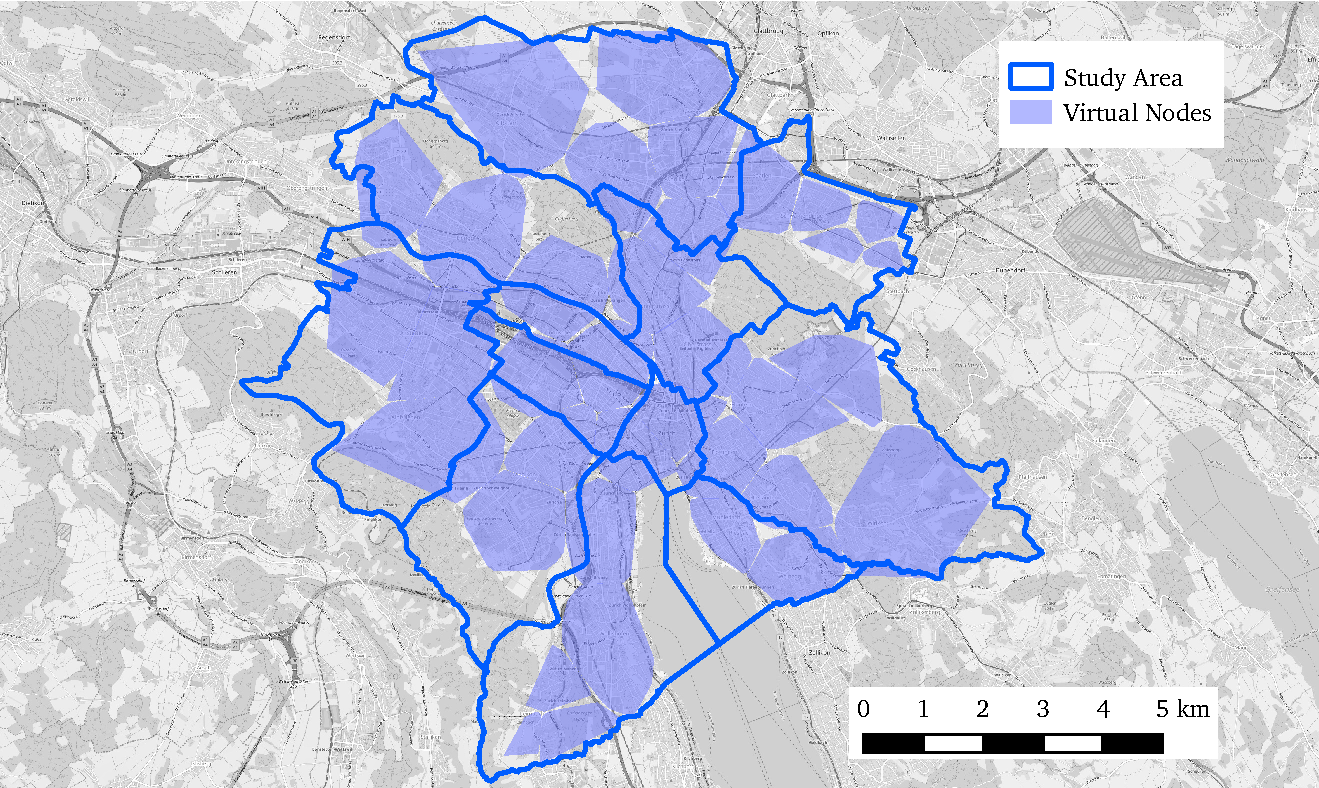
\includegraphics[width=1.0\textwidth]{figures/map.pdf}\end{center}
\caption{The study area covering the 12 districts of Zurich and the nodes of the
virtual network for the rebalancing algorithms.}
\label{fig:study_area_vnodes}
\end{figure}

Additional modifications are applied to this population of around 8 million
agents to make it suitable for the study at hand. First, a best-response routing
of the travels of all agents is performed to find all agents that interfere
with the study area, which has been defined to the 12 districts of Zurich (Figure \ref{fig:study_area_vnodes}).
All agents which do not interact with that region (performing an activity within
the area or crossing the area) are deleted from the population as they do
not contribute to the state of the traffic system in that area. Finally, a 1\%
sample of the remaining agents is created, which is the basis for our
simulations. The rather extensive downscaling becomes necessary for the computationally
demanding algorithms, given that they need to be performed hundreds of times faster
than reality to allow for multiple runs and iterations.

In order to define the travel demand for the fleet of automated vehicles, agents
are tagged as whether they are viable for using an automated vehicle or not. Pedestrians and cyclists are not simulated at all in this work since they do not contribute to congestion in the current version of the framework. 

An agent that travels at least once by private car during the simulation is tagged
as an AV user \textit{only} if all of the legs in the agent's plan take place
within the study area. This constraint makes sure that no unrealistic travel
plans are generated, where an agent performs his first leg by AV although his
private car is at home and then wants to depart at the next location with that
car. Finally, the ``car'' legs of all viable agents are converted to the ``av'' mode.
All other legs are kept as before, i.e. short legs that are assigned the ``walk''
mode initially are still performed in this mode.

For agents that use public transit, the procedure is different. Here, any leg
that is performed by the ``pt'' mode in the original population is converted to ``av''
if it lies within the study area. As for car users, connecting non-motorized
legs are kept fixed. Proceeding as outlined, a demand for Zurich is generated in which each leg that possibly
\textit{can} be performed using an AV \textit{is} performed by AV.

To summarize, the 8,230,971 agents in the population are reduced to
1,935,400 agents, which interfere with the study area. From this set of agents
a 1\% sample has is drawn, leading to 13,141 agents that mainly constitute
background traffic for congestion. Among those are 970 agents that are viable for the AV
service. The plans of these agents contain 2,096 trips that are to be served by
AVs. In reality, this service would hence need to serve 209,000 requests by
97,000 persons.

\subsection{Theoretical Fleet Sizing}

Both the capital cost of an AMoD system and the service rates are highly dependent
on the fleet size which makes fleet siziing an important aspect of AMoD system design.
If the fleet size is chosen too small, then the service levels will be inacceptable, if the fleet size is chosen too large, the cost of the system becomes unbearable due to low utilization rates.

Fleet sizes can be estimated using simulations, as for instance done in
\citep{bischoff2016simulation}. Despite of the accuracy of these
simulation results, they do not provide insights into the fundamental
properties influencing the relationship between fleet size and performance metrics.

For this reason we have implemented theoretical results from \citep{spieser2014toward}
for the case of Zurich. The authors present two methods for fleet size evaluation.
The first method estimates the theoretical minimum fleet size to stabilize
the system, i.e. ensure that the number of open requests stays bounded at
all times. To do so, for every vertex $i$ and timestep $\delta_t$ the added
unserved mileage per timestep is calculated as
$\lambda_i \cdot ( \bar{d}_{OD,i}  + \bar{d}_{EMD,i})$ where $\bar{d}_{OD,i}$
is the average distance per trip and  $\bar{d}_{EMD,i}$ the earth mover's
distance per vehicle in the timeslice. $\bar{d}_{OD,i}  + \bar{d}_{EMD,i}$
represents the average distance that has to be driven per request. A total of
$m$ vehicles at an average speed of $v$ are collectively able to reduce this
 added mileage at a rate of $m \cdot v$. This quantity has to be larger than the
 added unserved mileage per timestep. For the scenario of this work the
 minium fleet size compute with this measure are $1380$ vehicles. 

While the knoweldge of the minimum fleet size is useful, it does not reveal
the relation between service level and fleet size, especially to what number
the fleet size has to be augmented before further addition of vehicles will
not result in a significant increase in service level. In \citep{zhang2016control}
 a method is presented of how an AMoD system can be cast in a Jackson network.
 For such networks, queuing theoretical results allow the computation of
 performance measures such as vehicle wait times, queue lengths or
 availabilities at vertices. The quantity of interest is the availability
 of a vehicle at a vertex, which is the probability that $1$ or more idle
 vehicles are at that vertex. Computation of the mean availability of all
 timesteps and vertices as a function of the fleet size for Zurich results
 in the curve shown in \ref{fig:performanceavailability}. Note that these results are purely theoretical and can be derived solely from input data without performing simulations. Therefore they can serve
as a measure of accuracy for the simulation results.

\begin{figure}[h]
\begin{center}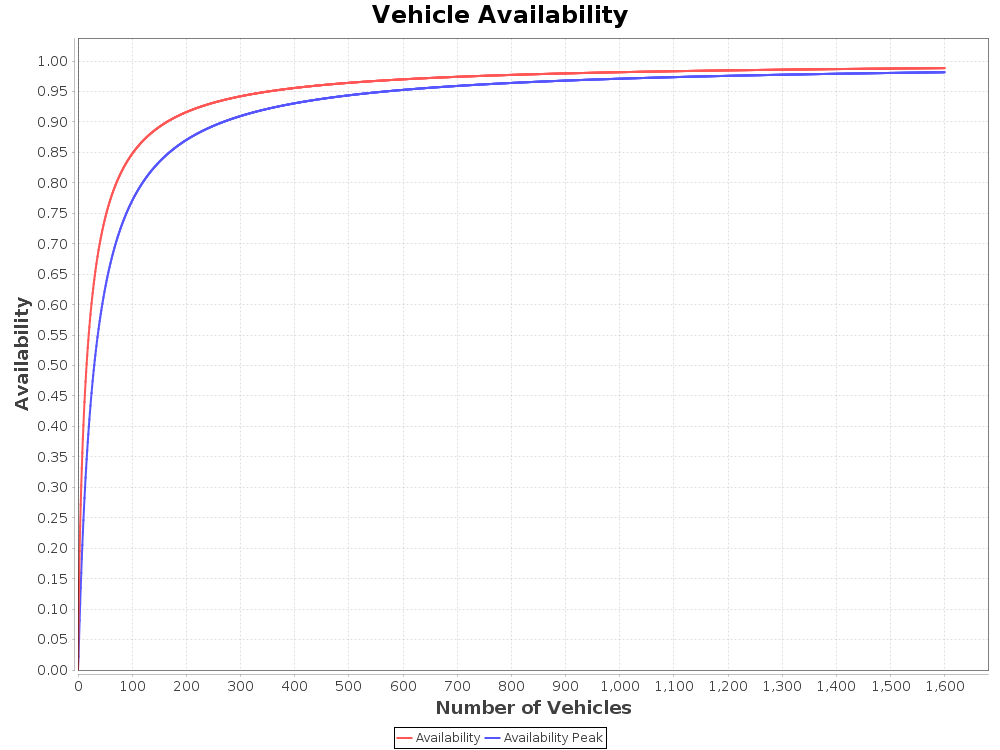
\includegraphics[width=1.0\textwidth]{figures/availbilitiesByNumberVehicles.png}\end{center}
\caption{Mean availability of vehicles over all timesteps and virtual vertices.  TODO correct plot with scaling x 100}
\label{fig:performanceavailability}
\end{figure}

For the peak case, the increase of the number of vehicles up to a fleet size of $15,000$ results
in a availability rising from $0$ to $~0.85$. The addition of another $15'000$ vehicles does only increase the availability by $~0.05$ to $~0.90$. This corresponds well to the wait times observed in simulation shown in figure \ref{fig:mean_peak_waiting_times}. The simulated wait times decrease significantly up to a fleet size of $15,000$ and further increase of the fleet size improves the wait times only insignificantly. 
\section{Simulations}
\label{sec:staticSimulations}

The dispatching algorithms as presented before have been tested in the agent-
and activity-based transport simulation framework MATSim. What has been used in
this paper is the mobility simulation component of that package, where each agent
has a daily plan consisting of activities and legs. Activities are performed for a
certain duration at specific locations in the traffic network and have predefined
end times. They are connected by legs, which are performed by specific means of
transport. Dependent on the time of day, the mode, the route taken and other factors,
travel times may vary. Most importantly, the network is capacitated such that
congestion emerges if many agents use the same networks links at the same time.

Most important for the study at hand is the simulation of vehicles in an actual
network. By keeping background traffic in the simulation, the AVs are constrained
by the network conditions, most remarkably they suffer from longer travel times
at peak hours due to congestion.

The section is divided into two parts: First, we describe how the simulation
scenario has been set up to account for a realistic travel demand for Zurich.
Second, the simulation approach for automated vehicles is explained and third,
the results for the different dispatching algorithms are presented.

\subsection{Scenario Setup}
\label{sec:simulations_scenario}

For Switzerland the Microcensus on mobility and transport \cite{microcensus} is
available, which features the daily travel patterns of 60,000 Swiss residents.
In a previous study it has been used to create a detailed agent population of
Switzerland, which reproduces the demographic attributes and travel patterns
in the country to great detail \cite{ivtbaseline}.

Additional modifications have been applied to this population of around 8 million
agents to make it suitable for the study at hand. First, a best-response routing
of the travels of all agents has been performed to find all agents that interfere
with the study area, which has been defined to the 12 districts of Zurich (Figure \ref{fig:study_area_vnodes}).
All agents which do not interact with that region (performing an activity within
the area or crossing the area) have been deleted from the population as they do
not contribute to the state of the traffic system in that area. Finally, a 1\%
sample of the remaining agents has been created, which is the basis for our
simulations to account for feasible computation times for the proposed dispatching
algorithms.

In order to define the travel demand for the fleet of automated vehicles, agents
have been tagged as whether they are viable for using an automated vehicle or not.
While pedestrians and cyclists have not been simulated at all (since they do not
contribute to congestion in the current version of the framework), agents that
travel by car or public transit at least once during their daily plan are
handled differently.

Agents that travel at least once by private car during the simulation are tagged
as an AV user \textit{only} if all of the legs in the agent's plan take place
within the study area. This constraint makes sure that no unrealistic travel
plans are generated, where an agent performs his first leg by AV although his
private car is at home and then wants to depart at the next location with that
car. Finally, the ``car'' legs of all viable have been converted to the ``av'' mode.
All other legs are kept as before, i.e. short legs that were assigned the ``walk''
mode before are still performed in this mode.

For agents that use public transit, the procedure is different. Here, any leg
that is performed by the ``pt'' mode in the original population is converted to ``av''
if it lies within the study area of 15km. As for car users, connecting non-motorized
legs are kept fixed.

This way a demand for Zurich has been generated where each leg that possibly
\textit{can} be performed using an AV \textit{is} using an AV. In that sense we
simulate a scenario where 100\% of the AV travel demand must be served by the
dispatchers.

To summarize, the 8,230,971 agents in the population have been decimated to
1,935,400 agents, which interfere with the study area. From this set of agents
a 1\% sample has is drawn, leading to 19,354 agents that mainly constitute
background traffic. Among those are 970 agents that are viable for the AV
service. The plans of these agents contain 4030 trips that are to be served by
AVs. In reality, this service would hence need to serve 403,000 requests by
97,000 persons.

\subsection{Simulation of automated vehicles}

To simulate automated vehicles in the MATSim scenario, a framework extension by
Hörl \cite{horl_abmtrans17} is used. There, AVs are individually simulated on the
road network, contributing to and experiencing congestion. As soon as agents
finish their activities the simulation is notified about an incoming request
given that the agent wishes to use an AV for the following leg. In that case
the request with its properties (departure time, origin, destination) is passed
on to the dispatcher. These dispatchers are based on different algorithms, as
described before. However, the ``lifecycle'' of a request is always the same: First,
an AV needs to drive to the location of the customer, pick him up, drive to the
final location and finally drop the customer off. From the point a customer has
been picked up, the process is predetermined, no changes to the route of the AV
are made anymore. While an AV has been assigned to a customer for pickup the
vehicle may be reassigned depending on the dispatching algorithm.

It should be noted that AVs drive directly to the locations where agents end and
start their activities. So far no mechanism is implemented that would allow them
to meet at optimized locations (e.g. a high-capacity avenue instead of a small
alley).

\section{Results}
\label{sec:results}

We test the four proposed dispatching strategies in the Zurich scenario with four runs per strategy. Each run simulates 20 iterations to allow the dispatchers to sense the traffic conditions in the network, i.e. to figure out what travel times on specific links are expected and how traffic jams can be avoided.

For Zurich, the times with peak congestion and, hence, longest travel times are from 6:30am to 9:00am and from 4:30pm to 6:30pm. In figure \ref{fig:mean_peak_waiting_times} all trips by AV with departures times in these time windows are collected and the mean waiting time for vehicle is computed. As expected, the average waiting time is decreasing with larger fleet sizes and higher availabiltiy of vehicles. Almost over the whole range of flet sizes the feedback LP dispatcher performs best, while the load-balancing heuristic features the longest waiting times.

\begin{figure}
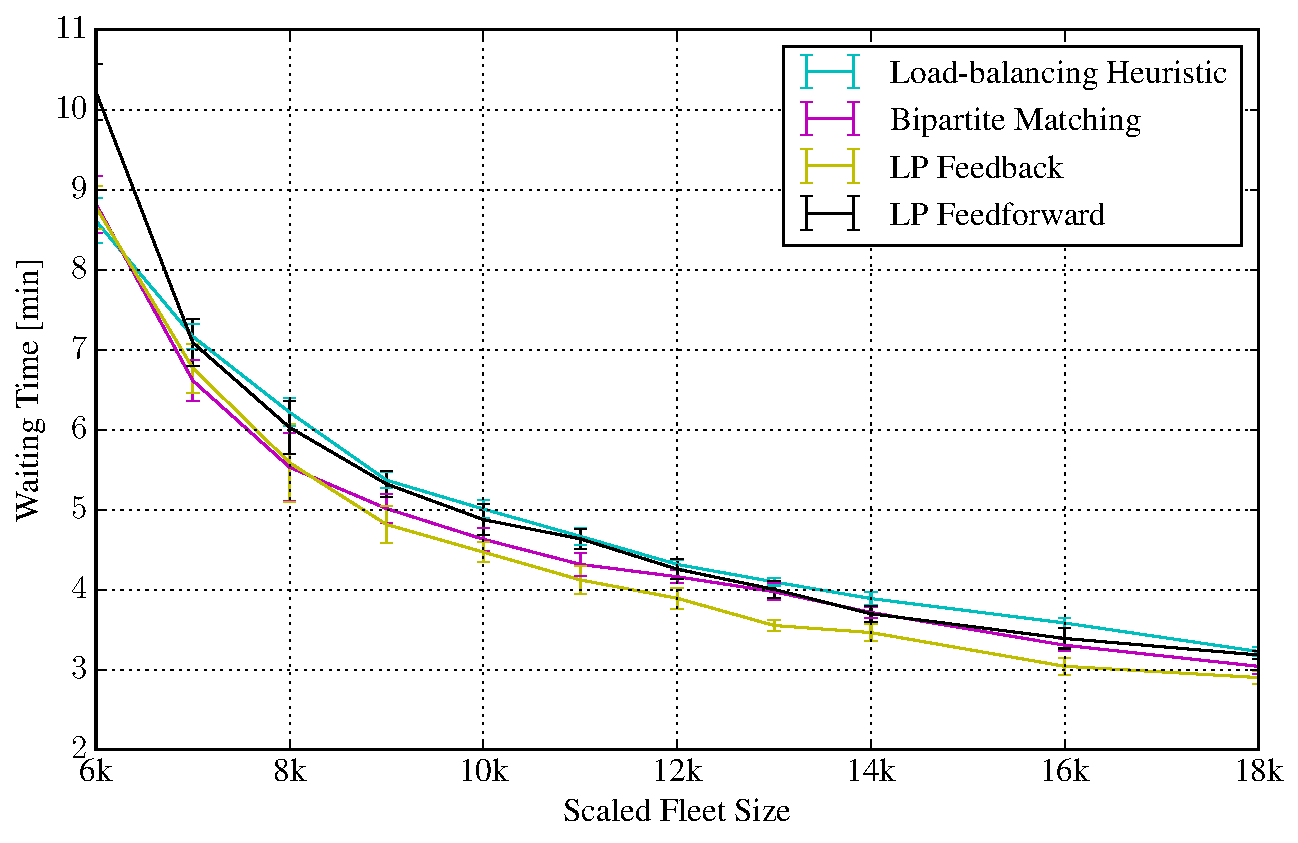
\includegraphics[width=1.0\textwidth]{figures/mean_peak_waiting_times.pdf}
\caption{Average waiting time for an AV to arrive at peak times}
\label{fig:mean_peak_waiting_times}
\end{figure}

Figure \ref{fig:empty_rides} shows the percentage of fleet mileage that is driven without a customer, either for pickup or rebalancing purposes. Clearly, the LP algorithms, which both use rebalancing, have a higher share of empty mileage that the non-rebalancing approaches. The heuristic approach manages to keep the share lowest, since it mainly operates in a best-response state, where only the shortest pickup trips are chosen. Remarkably, the total driven distance for all dispatchers is very similar (Figure \ref{fig:total_distance}), which indicates that the surplus of empty distance for the intelligent dispatchers does not stem from inefficient movements, but rather effective movements towards the expected customer demand for shorter waiting times.

[TODO: Do we need two plots here? Also a plot Total Distance <-> Relative Distance
would be possible, where one can traverse the fleet size along the graph]

\begin{figure}
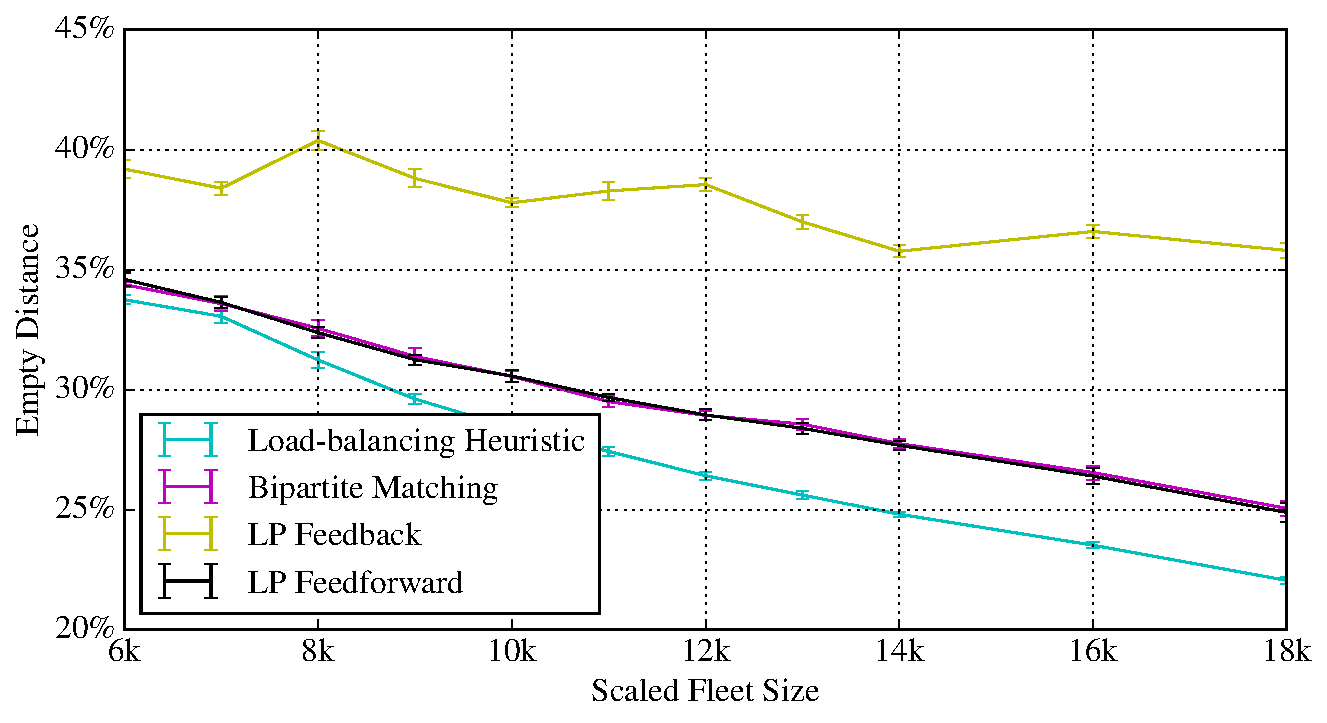
\includegraphics[width=1.0\textwidth]{figures/empty_rides.pdf}
\caption{The fraction of distance that is driven by AVs without a passenger.}
\label{fig:empty_rides}
\end{figure}

\begin{figure}
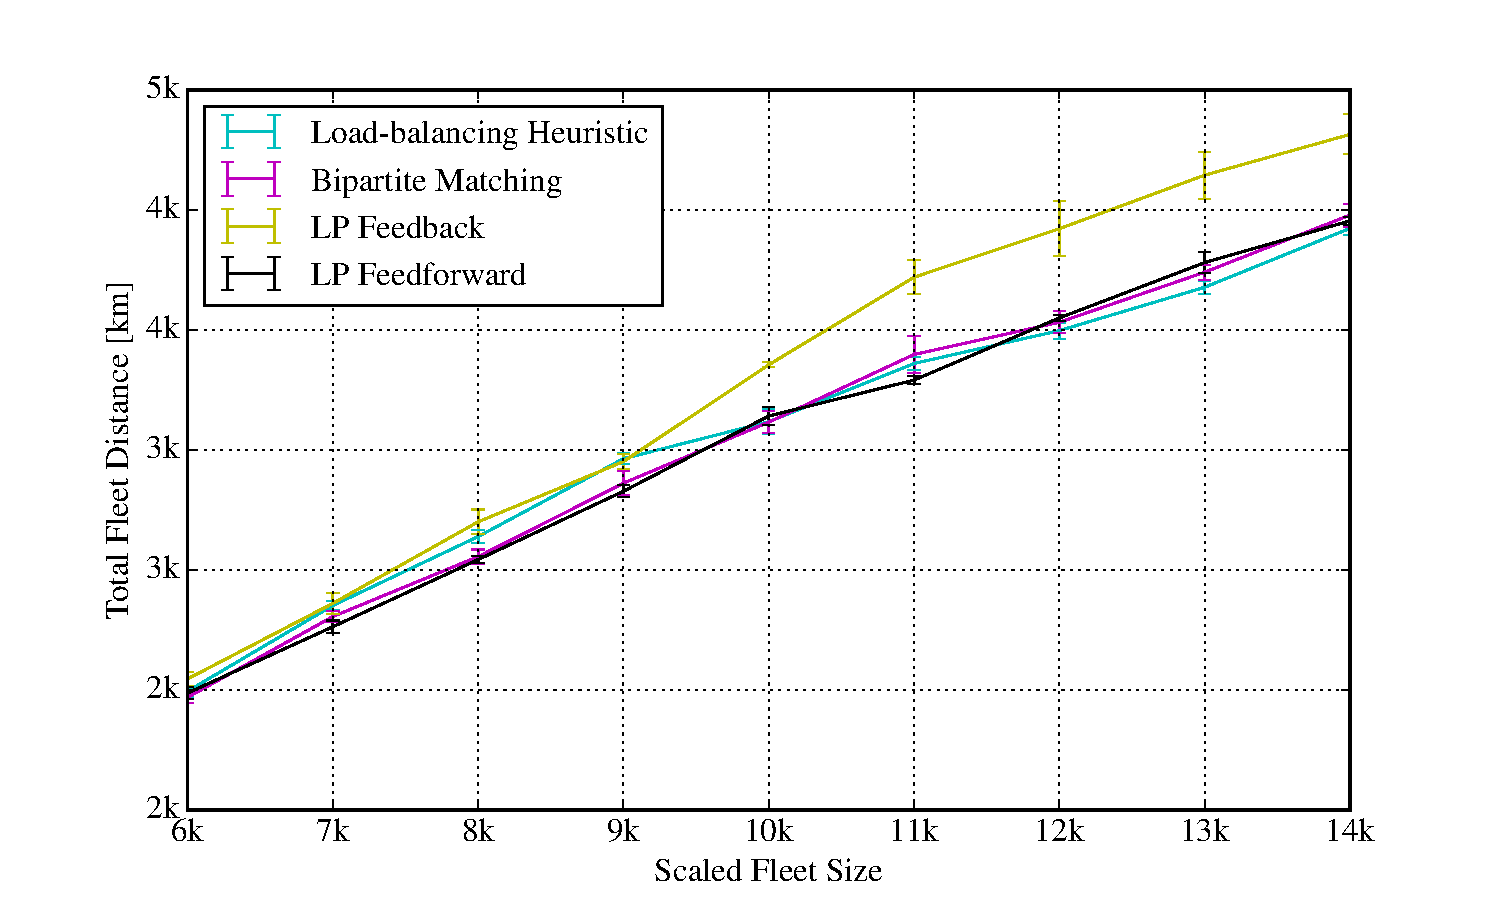
\includegraphics[width=1.0\textwidth]{figures/total_distance.pdf}
\caption{The total distance that is driven by AVs, with and without passenger on-board.}
\label{fig:total_distance}
\end{figure}

Finally, figure \ref{fig:occupancy} shows the occupancy of the fleet for different fleet sizes. Since in the 30h MATSim simulation no AV trips are registered in the hours around midnight, it is possible to correct the resulting 30h occupancy rate to one that is based on a 24h day. As can be seen, the occupancy of all fleet dispatchers exceeds the 8\% that is common today. In general, one can say that the dispatching algorithm has only little influence on fleet occupancy
 [TODO: Trips and Costs are fixed!!]
. The differences lie in the range of 0.5\% between the best and worst performing algorithm, which are the LP Feedback dispatcher and the load-balancing heuristic, respectively. Nevertheless, one can see that the occupancy of the latter is systematically lowest.

\begin{figure}
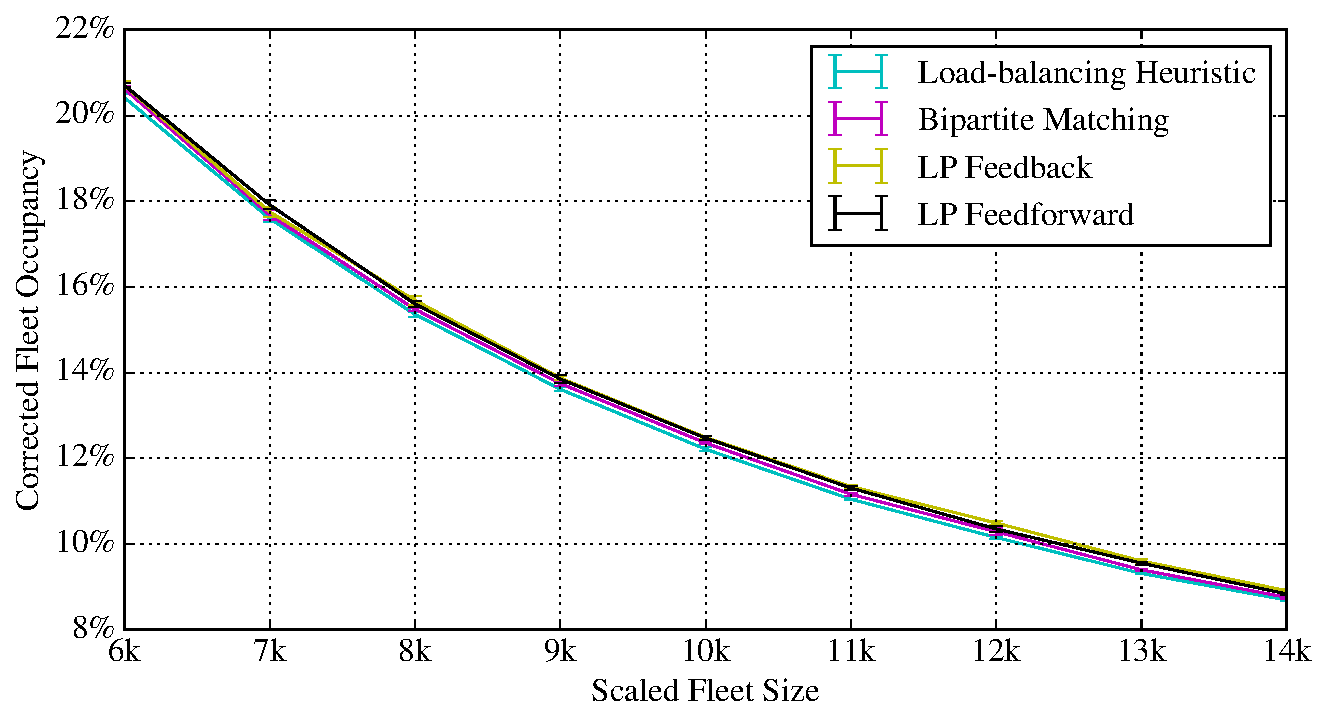
\includegraphics[width=1.0\textwidth]{figures/occupancy.pdf}
\caption{The occupancy of the AV fleet for different flet sizes.}
\label{fig:occupancy}
\end{figure}

\subsection{Cost Analysis}
\label{sec:cost_analysis}

Based on a paper Bösch et al. \cite{cost_paper} the costs of operating the simulated AV services are computed. Specifically, by providing their calculator with key figures of the operator (among them the occupancy, the share of empty rides, the average travel distance) the price that the operator would at least need to ask a customer per kilometer if a profit margin of at least 3\% is targeted. The calculation is based on a detailed analysis of running and fixed costs. Figure~\ref{fig:passenger_price} shows the results from this analysis. Unsurprisingly, the price that needs to be imposed on the customer increases with larger fleet sizes. However, the increase is stronger for the load-balancing heuristic than for any other distpaching strategy. Therefore, with the same fleet being available to an operator, he would be able to offer the service for almost 0.10 CHF less per kilometer than before or save this amount of money.

\begin{figure}
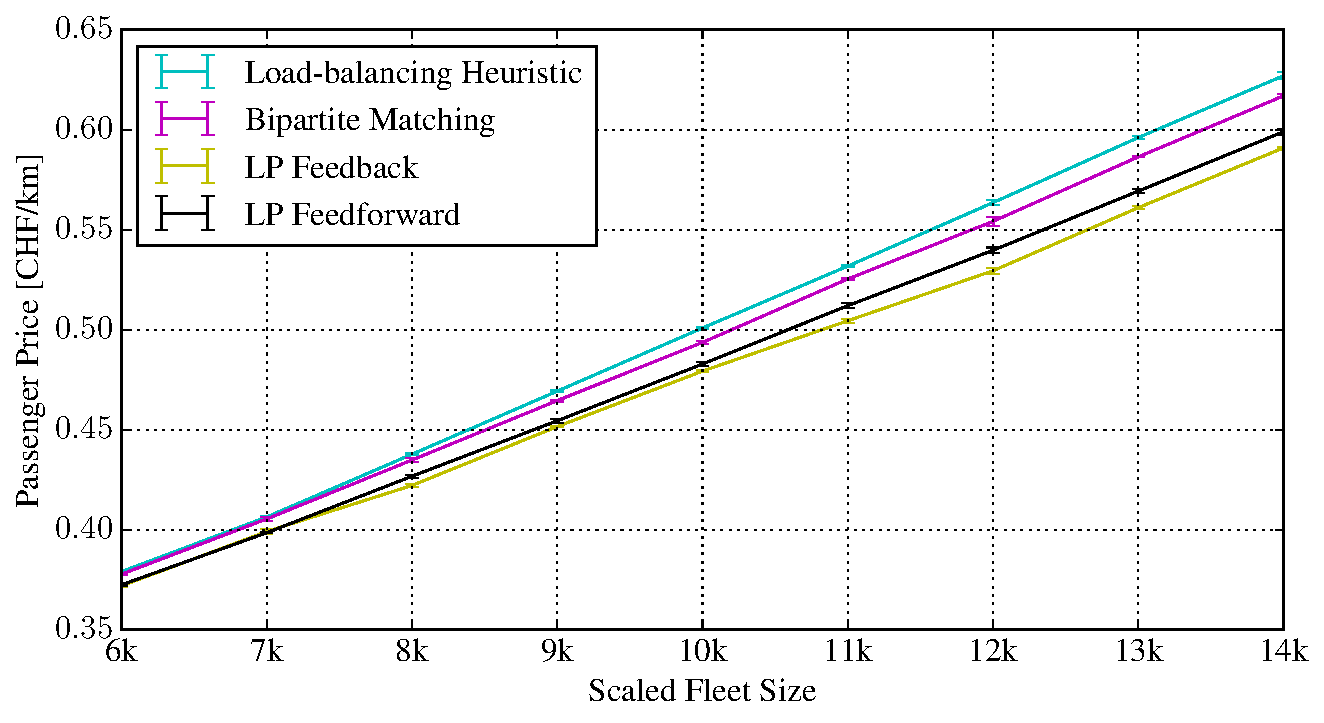
\includegraphics[width=1.0\textwidth]{figures/01_passenger_price.pdf}
\caption{The minimum customer prices that an AV operator needs to charge the customer
in order to have a win margin of at least 3\%.}
\label{fig:passenger_price}
\end{figure}

Compared to the average running costs of driving a private car in Switzerland (around 0.17 CHF/km) 

[todo{variable.. full costs present a nicer story] 

or using public transit (around 0.25 CHF/km) [TODO CITATIONS] the computed prices still seem rather high. Compared to conventional taxi operators, however, the price is extremely low (around 6 CHF/km). Therefore, it is imaginable that the AV service would still be attractive for a large group of people, for which a conventional taxi would be too expensive on a daily basis, but an AV would make such travels affordable.

However, the attractiveness of an AV service does not only depend the price itself, but also on the attitudes of the people towards the service. One key component to the acceptance of an AMoD system is the waiting times that customers need to endure. Figure \ref{fig:time_vs_price} combines the key results from our simulations. There, the price that a specific operator configuration (fleet size and dispatcher) is displayed in comparison to the waiting time that this operator can offer. Assuming that, for instance, a waiting time of five minutes is tolerable, the operator could offer a satisfactory service for around 0.45 CHF with the feedback dispatcher, while he would need to charge 0.50 CHF with the simple load-balancing heuristic. The better the level of service of the operator is ought to be, the larger this margin becomes.

\begin{figure}
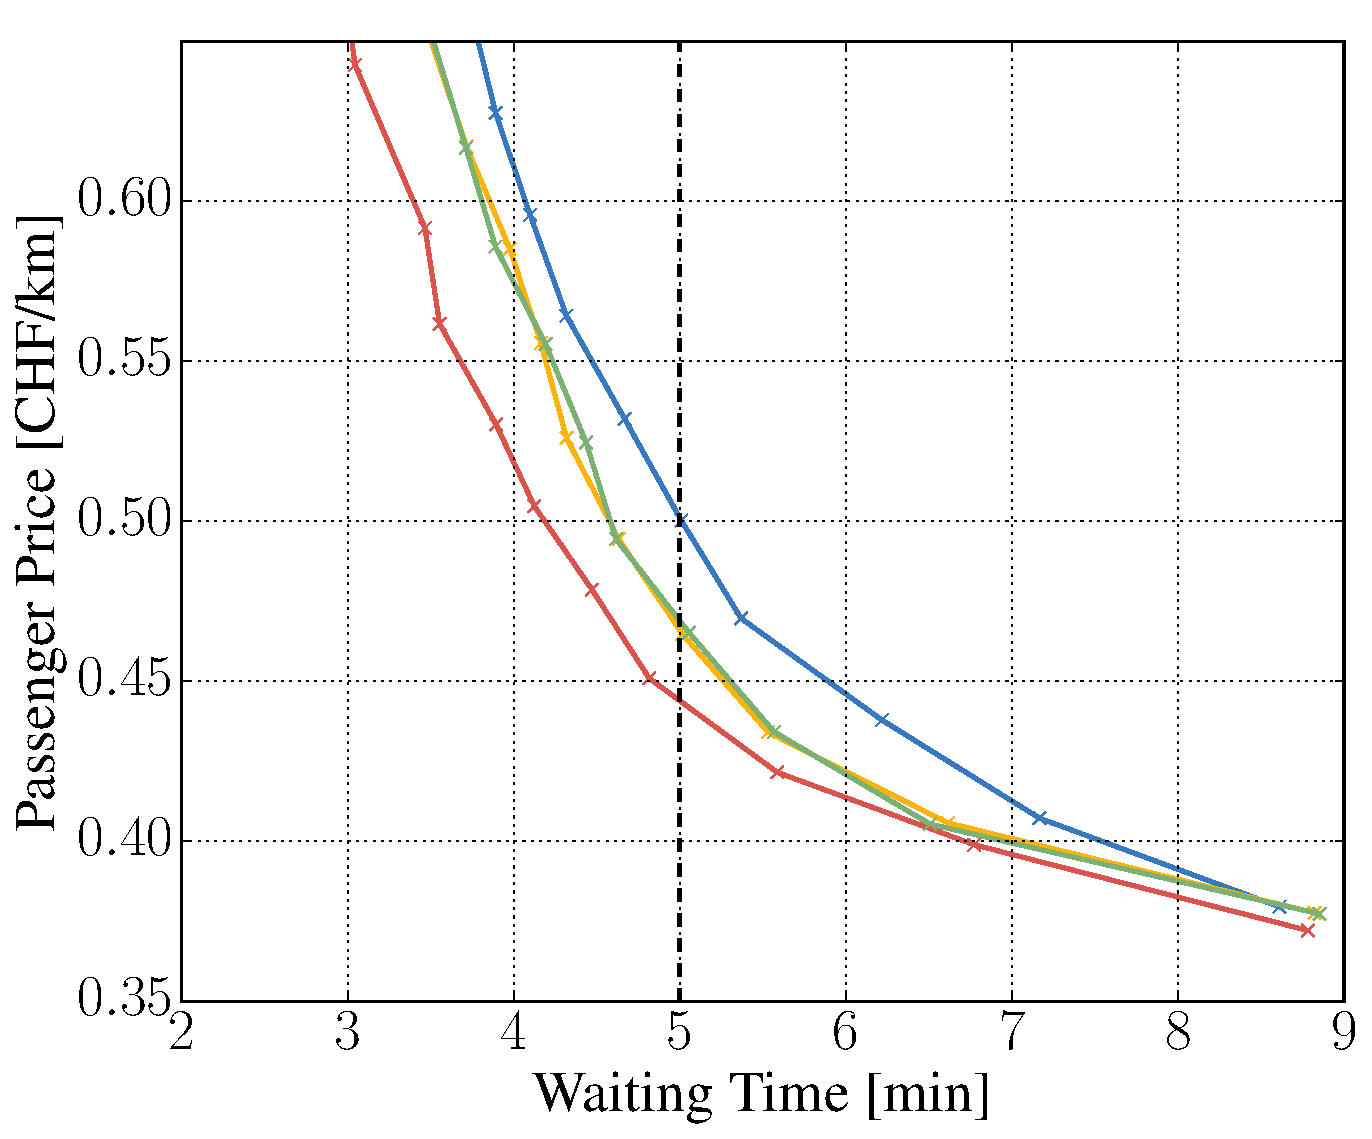
\includegraphics[width=1.0\textwidth]{figures/time_vs_price.pdf}
\caption{Time vs. Price}
\label{fig:time_vs_price}
\end{figure}

\section{Discussion \& Conclusion}
\label{sec:Conclusion}

The study shows that the right choice of dispatching algorithm for an AMoD system does not only have a strong impact on the performance in terms of waiting times for the customer but also that it bears a substantial economic advantage for the
operator. He is able to attract more customers through quicker pickups and lower prices than a competitor with only little investment.

In order to assess the significance for real fleets of (not necessarily
automated) taxis it needs to be noted that all of the presented algorithms are able to process dispatching and rebalancing tasks for fleets of thousands of vehicles within minutes. It is perfectly feasible to control 100k vehicles in five minute updates using a standard laptop for the computational tasks.

For the presented simulations, this still poses a burden, though,  because there a speedup compared to the reality of around one thousand times is desired to be able to run large numbers of simulations with different parameters. Hence, the algorithms
could only be tested on a subsample of 1\% of the agent population that is available. In future studies effort will be put into overcoming these restrictions, either by finding approximate formulations for the presented algorithms or pursuing research on completely new algorithms.

Throughout the paper, a ``100\%'' demand scenario has been used, in which all trips that possibly could be undertaken by AV were converted to the automated mode. The MATSim framework, however, offers the possibility to explicitly simulate attitudes toward new elements in the traffic system by defining utilities for using specific modes with a distinct valuation of travel costs, travel times and distances. This way, by integrating the presented algorithms into the full MATSim loop as shown in \cite{horl_abmtrans17} the actual attractiveness of an AV service could be analyzed including the tradeoff that people make between paying for the service, spending time in the vehicle and having to wait for it.
Naturally, not 100\% of possible trips would actually be performed by AV, but only a fraction. In such a scenario, also if maybe more remote areas would be included, completely different properties of an AV fleet control algorithm would be of interest, e.g. how well it is able to attract new customer groups in new regions by offering unproportionally low waiting times and make them stick to the service.


%\input{Background}
%\input{ScoringMATSim}
%\input{ProposedScoringFunction}
%\input{DefaultProposedUtilityFunction}
%\input{ReschedulingResults}
%\input{Discussion}
%\input{Conclusion}
%%%%%%%%%%%%%%%%%%%%%%%%%%%%%%%%%%%%%%%%%%%%%%%%%%%%%%%%%%%%%%%%%%%%%%
%% Bibliography
%%   Leave this as is, and add you own entries to my.bib
%%   Many references are already defined in _latexfiles/bibs/all-eng.bib
%%   Refer to the BibTeX/LaTeX tutorial for adding new entries
%%   to the IVT BibTeX database
\bibliography{\mypath/bibs/all-eng,my}
%%%%%%%%%%%%%%%%%%%%%%%%%%%%%%%%%%%%%%%%%%%%%%%%%%%%%%%%%%%%%%%%%%%%%%

%%%%%%%%%%%%%%%%%%%%%%%%%%%%%%%%%%%%%%%%%%%%%%%%%%%%%%%%%%%%%%%%%%%%%%
%% Appendices
%%   Usually they would start on a separate page
%%%%%%%%%%%%%%%%%%%%%%%%%%%%%%%%%%%%%%%%%%%%%%%%%%%%%%%%%%%%%%%%%%%%%%


\end{document}

%%%%%%%%%%%%%%%%%%%%%%%%%%%%%%%%%%%%%%%%%%%%%%%%%%%%%%%%%%%%%%%%%%%%%%
%%%%%%%%%%%%%%%%%%%%%%%%%%%%%%%%%%%%%%%%%%%%%%%%%%%%%%%%%%%%%%%%%%%%%%
%%
%% END OF DOCUMENT
%%
%%%%%%%%%%%%%%%%%%%%%%%%%%%%%%%%%%%%%%%%%%%%%%%%%%%%%%%%%%%%%%%%%%%%%%
%%%%%%%%%%%%%%%%%%%%%%%%%%%%%%%%%%%%%%%%%%%%%%%%%%%%%%%%%%%%%%%%%%%%%%

%%%%%%%%%%%%%%%%%%%%%%%%%%%%%%%%%%%%%%%%%%%%%%%%%%%%%%%%%%%%%%%%%%%%%%
%% Editor specific keywords:
%%   This is not part of you paper, but sometimes it is used
%%   for additional features of TeX Editors.
%%
%% WinEdt:
%%   to get the bibliography list
%GATHER{./_bibs/all-eng.bib}
